\documentclass[lang=cn,15pt]{elegantbook}
\usepackage{graphicx}
\usepackage{float}

\title{量子力学}



\author{Huang}
\date{\today}




\setcounter{tocdepth}{3}


\cover{cover.jpg}

% 本文档命令
\usepackage{array}
\newcommand{\ccr}[1]{\makecell{{\color{#1}\rule{1cm}{1cm}}}}

% 修改标题页的橙色带
% \definecolor{customcolor}{RGB}{32,178,170}
% \colorlet{coverlinecolor}{customcolor}

\begin{document}
	
	\maketitle
	\frontmatter
	
	\tableofcontents
	
	\mainmatter
\chapter{基本概念}
\section{何为量子}

场的最小激发是量子

最小激发有两层含义$\begin{cases}
	1.\text{场的激发不能无限小,必须有一个最小单元}\\
	2.\text{量子不可分}\\
\end{cases}$

这就导致了量子世界的分立性

因此量子代表了一种观点,即——\textbf{世界不是连续的,而是分立的}
\section{简单历史}
\subsection{经典理论遇到的问题——黑体辐射}

\textbf{黑体}:能吸收外来的全部电磁辐射,不发生反射和投射

\textbf{黑体辐射}:黑体会发出热辐射,其光谱特征仅与黑体的温度有关,与黑体的材质,大小形状均无关系

实验测得:

\begin{figure}[H]
	\centering
	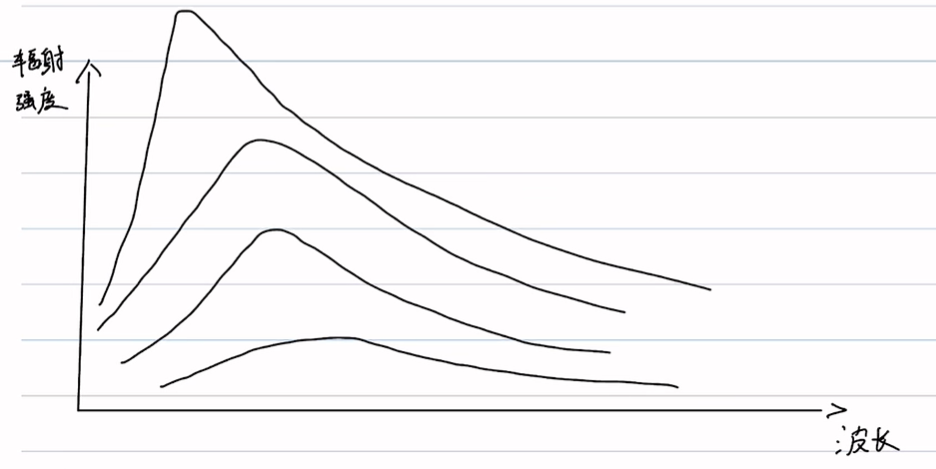
\includegraphics[width=0.5\linewidth]{figure/screenshot001}
\end{figure}

使用$\mathop {\underbrace{\text{经典理论}}} \limits_{\text{能量连续}}$公式的wien,Rayleigh和Jeans都失败了

以Rayleigh-Jeans公式为例,它以能量均分定律(每一个自由度吸收$\frac{1}{2}kT$的能量)为基础,给出
\begin{equation}
	I\left( \omega \right) =\frac{\omega ^2}{\pi ^2c^2}kT
\end{equation}
这个公式在$\omega$较大时候会快速发散

Plunk先从插值法通过Wien公式和Rayleigh-Jeans公式拟合出了Plunk公式
\begin{equation}
	I\left( \omega \right) =\frac{1}{e^{\frac{a\omega}{\mu T}}}\cdot \frac{b\omega ^2}{\pi ^2c^2}\left( a,b\text{为常数} \right) 
\end{equation}
这与实验数据完全符合

接着,他开始思考为什么正确的公式会是这样

他发现左边的像Bolztmann分布
\begin{equation}
	N_n=N_1e^{-\frac{\left( E_n-E_1 \right)}{kT}}
\end{equation}

因此他大胆假设,辐射场中的偶极振子的能量是\textbf{一份一份的}(不连续、分立)

每份的能量依赖其角频率
\begin{equation}
	E=a\omega
\end{equation}

带有每种能量的偶极子的数目服从Boltzmann分布
\begin{equation}
	\begin{split}
		N_n=&N_0e^{-\frac{E_n}{kT}}\\
		&N_0e^{-\frac{n\omega}{kT}}
	\end{split}
\end{equation}

平均能量\begin{equation}
	\begin{split}
		\left< E \right> &=\frac{E_{\text{总}}}{N_{\text{总}}}=\frac{\sum_n{N_n\cdot E_n}}{\sum_n{N_n}}=\frac{\sum_n{N_0\cdot e^{-\frac{na\omega}{kT}}\cdot na\omega}}{\sum_n{N_0\cdot e^{-\frac{na\omega}{kT}}}}
		\\
		&=\frac{a\omega \left( 0\cdot e^{-\frac{0a\omega}{kT}}+1\cdot e^{-\frac{a\omega}{kT}}+2\cdot e^{-\frac{2a\omega}{kT}}+3\cdot e^{-\frac{3a\omega}{kT}}+\cdots \right)}{1+e^{-\frac{a\omega}{kT}}+e^{-\frac{2a\omega}{kT}}+e^{-\frac{3a\omega}{kT}}+\cdots}
		\\
		&=\frac{a\omega \left( \varepsilon +\varepsilon ^2+\varepsilon ^3+\cdots \right)}{1+\varepsilon +\varepsilon ^2+\varepsilon ^3+\cdots}\left( \text{令}\varepsilon =e^{-\frac{a\omega}{kT}} \right) 
		\\
		&=\frac{a\omega \varepsilon \frac{d}{d\varepsilon}\left( 1+\varepsilon +\varepsilon ^2+\varepsilon ^3+\cdots \right)}{1+\varepsilon +\varepsilon ^2+\varepsilon ^3+\cdots}
		\\
		&=\frac{a\omega \varepsilon \frac{d}{d\varepsilon}\frac{1}{1-\varepsilon}}{\frac{1}{1-\varepsilon}}
		\\
		&=a\omega \varepsilon \frac{1}{1-\varepsilon}
		\\
		&=a\omega \frac{e^{-\frac{a\omega}{kT}}}{1-e^{-\frac{a\omega}{kT}}}
		\\
		&=a\omega \frac{1}{e^{\frac{a\omega}{kT}}-1}
		\\
	\end{split}
\end{equation}

由此,由Rayleigh——Jeans公式中的平均能量$kT$被$a\omega \frac{1}{e^{\frac{a\omega}{kT}}-1}$取代
\begin{equation}
	\begin{split}
		I\left( \omega \right) &=\frac{\omega ^2}{\pi ^2c^2}a\omega \frac{1}{e^{\frac{a\omega}{kT}}-1}
		\\
		&=\frac{1}{e^{\frac{a\omega}{kT}}-1}\frac{a\omega ^3}{\pi ^2c^2}
		\\
	\end{split}
\end{equation}
其中的$a$就是如今的约化Plunk常量$\hbar $
\begin{equation}
		I\left( \omega \right)=\frac{1}{e^{\frac{\hbar\omega}{kT}}-1}\frac{a\omega ^3}{\pi ^2c^2}
\end{equation}
以上就为Plunk公式
\subsection{Einstein和光电效应}
\begin{figure}[H]
	\centering
	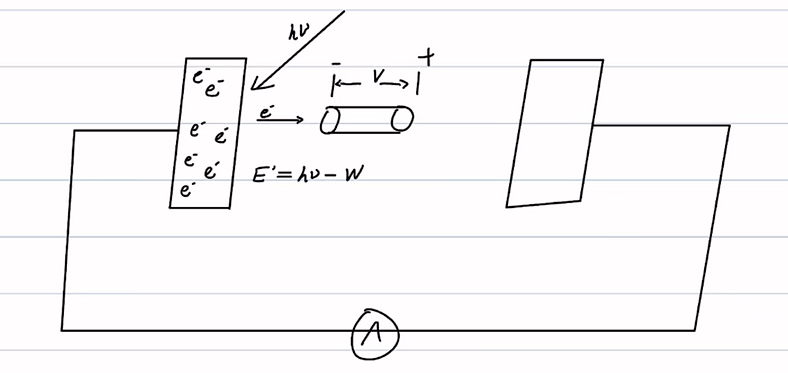
\includegraphics[width=0.8\linewidth]{figure/screenshot002}
\end{figure}

实验发现,光打在金属上会使电流表有示数,且对于单色光,只有特定频率以上的光才能使电流表有示数

Einstein利用Plunk的假说提出光是由一份一份的能量子/光量子构成的

\begin{enumerate}
	\item 每份光量子的能量为$h\nu$($\hbar\omega$)
	\item 光量子具有“整体性”,一个光量子只能整个地被电子吸收
\end{enumerate}

只有$h\nu$大于金属表面的逸出功时才能产生光生电流

对于光量子,我们有
\begin{enumerate}
	\item $E=h\nu$
	\item $E^2=m^2c^4=m_0^{2}+(pc)^{2}$
	\item $E=pc\rightarrow p=\frac{h\nu}{c}=\frac{h}{\lambda}$
\end{enumerate}
\subsection{波粒二象性}
\subsubsection{comptom效应}
\begin{figure}[H]
	\centering
	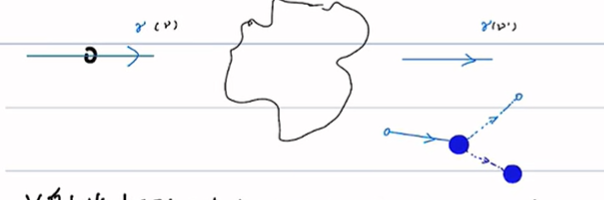
\includegraphics[width=0.7\linewidth]{figure/screenshot003}
\end{figure}
X射线打到碳靶上后部分散射光波变长

这用经典的光学无法解释,因为在经典光学中光在散射前后频率不变

但只要把光当成一份一份的光子具有动量和能量

光子与介质中的电子发生碰撞损失动量$p\rightarrow p'$变小,则$\lambda'=\frac{h}{p'}$变大

因此光不但具有波动性,还具有粒子性

\subsubsection{实物粒子的波粒二象性——deBrogile波}
既然长久被大量实验和完备的Maxwell方程组所支持的“光是波”的观点已经被打破,光具有粒子性,那么凭什么实物粒子反过来不能是波呢?

出于对物理对称性的尊重,deBrogile大胆提出所有的实物粒子都具有波动性,其波长$
\lambda=\frac{h}{mv^2}$
\subsection{Schrödinger方程}
Schrödinger根据光的波动方程和deBrogile的波粒二象性

猜测出了实物粒子的波动方程

电磁波
\begin{equation}
	\varphi =Ae^{i\left( kx-\omega t \right)}
\end{equation}

实物粒子
\begin{enumerate}
	\item $E=\hbar\omega$
	\item $k=\frac{2\pi}{\lambda}=\frac{2\pi}{h}p=\frac{p}{\hbar}$
\end{enumerate}

自由实物粒子
\begin{equation}
	\psi =Ae^{\frac{i}{\hbar}\left( px-Et \right)}
\end{equation}

则
\begin{equation}
	\frac{\partial \psi}{\partial t}=-\frac{i}{\hbar}Ae^{\frac{i}{\hbar}\left( px-Et \right)}\rightarrow i\hbar \frac{\partial \psi}{\partial t}=E\psi 
\end{equation}

而
\begin{equation}
	\begin{split}
		\frac{\partial ^2\psi}{\partial x^2}&=\left( -\frac{1}{i\hbar}p \right) ^2Ae^{\frac{i}{\hbar}\left( px-Et \right)}
		\\
		&=\left( -\frac{1}{i\hbar}p \right) ^2\psi 
		\\
		&=\left( -\frac{1}{i\hbar} \right) ^22\mu E\psi 
	\end{split}
\end{equation}


\begin{equation}
	\frac{1}{2\mu}\left( -i\hbar \frac{\partial}{\partial x} \right) ^2\psi =E\psi 
\end{equation}

于是

\begin{equation}
	\begin{split}
		i\hbar \frac{\partial}{\partial t}\psi &=\frac{1}{2\mu}\left( -i\hbar \frac{\partial}{\partial x} \right) ^2\psi 
		\\
		&=\hat{H}\psi \left( \hat{H}=\frac{1}{2\mu}\left( -i\hbar \frac{\partial}{\partial x} \right) ^2\text{称为}Hamilton\text{量} \right) 
	\end{split}
\end{equation}
\subsection{波函数的意义}
玻恩的统计诠释:因为光波的模平方等于光强,表示光子在该处的密度大小,因此对实物粒子也一样,波函数的模平方表示实物粒子出现在该处的概率密度大小

波函数本省则为概率振幅,没有确切的物理意义

这个性质要求$\int_{-\infty}^{+\infty}{|\psi |^2}=1$,因为概率总和为1,称为归一化条件
\subsection{态叠加原理$\&$量子态的坍缩}
\subsubsection{轻机枪氏双缝}
\begin{figure}[H]
	\centering
	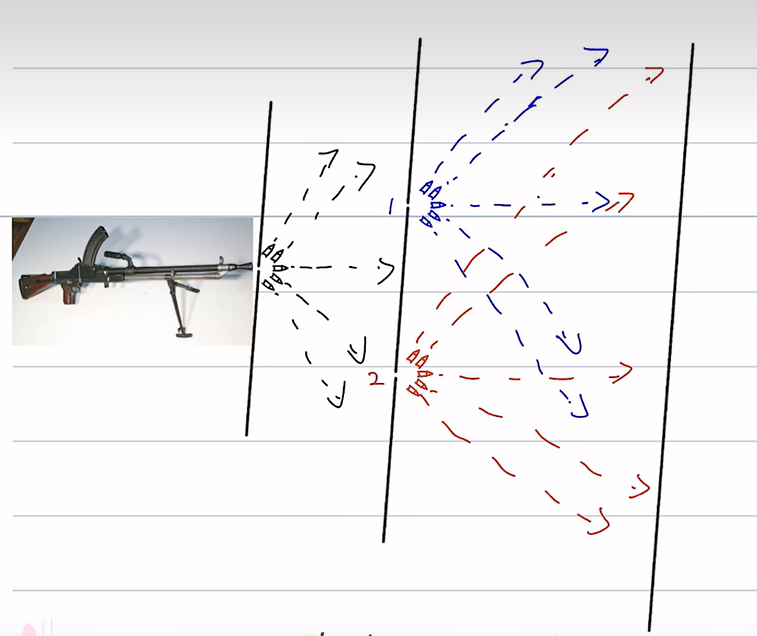
\includegraphics[width=0.7\linewidth]{figure/screenshot004}
\end{figure}
子弹总是一个个地打到接收屏上,我们统计大量子弹的最终分布
\subsubsection{水波双缝}
\begin{figure}[H]
	\centering
	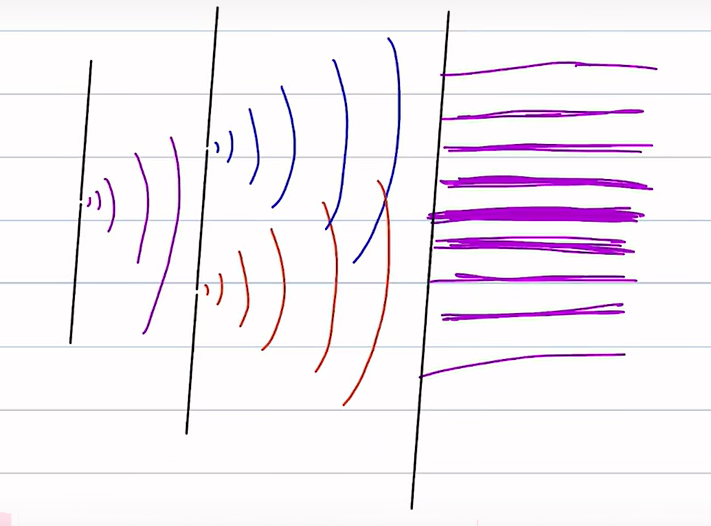
\includegraphics[width=0.7\linewidth]{figure/screenshot005}
\end{figure}
\subsubsection{电子双缝干涉}
\begin{figure}[H]
	\centering
	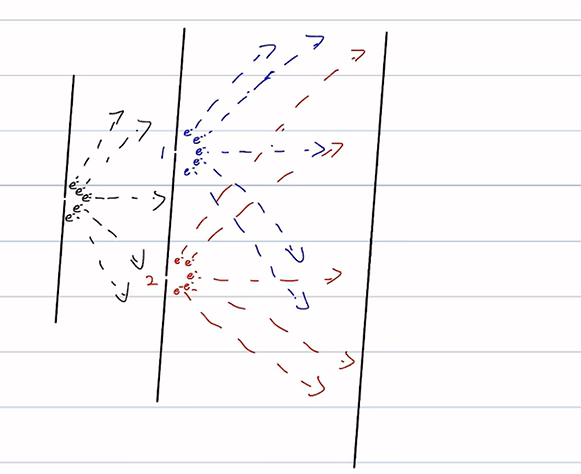
\includegraphics[width=0.7\linewidth]{figure/screenshot006}
\end{figure}
我们发现,无论是开几个缝,总是一个个的在屏上接收到粒子
\begin{figure}[H]
	\centering
	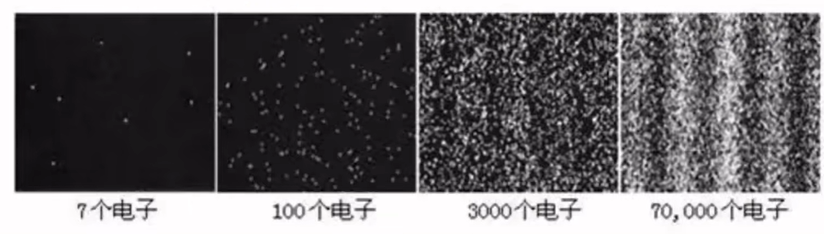
\includegraphics[width=0.7\linewidth]{figure/screenshot007}
\end{figure}

所以电子同时具有粒子性和波动性

现在我们做出总结
\begin{enumerate}
	\item 电子是以粒子的形式到达接收屏
	\item 电子在屏上出现的概率类似于波的干涉
\end{enumerate}
所以这种波描述的是电子出现在某处的概率密度

类比光的干涉,这种概率应正比于波在该处模场的平方$|\psi|^2$

我们称这种波为电子的概率波

现在,新的问题在于,一次发射一个电子也能产生干涉花样

所以电子是怎样通过双缝的?
\begin{enumerate}
	\item 一次通过一个缝?
	\item 同时出现在两个缝?
\end{enumerate}
答案是:电子以概率波的形式同时穿过两个缝并产生干涉,当落在光屏上又坍缩为粒子

设电子通过缝1的状态为$\psi_1$,通过缝2的状态为$\psi_2$,称为本征态(某个量确定的态称为本征态),则通过双缝后的粒子处于态
\begin{equation}
	\psi=c_1\psi_1+c_2\psi_2\quad\text{其中}|c_1|^2+|c_2|^2=1,\text{常系数}
\end{equation}
称为叠加态

当观测时,会以$|c_1|^2$的概率落入$\psi_1$态,以$|c_2|^2$的概率落入$\psi_2$态,并一直保持在这个态上,称为量子态坍缩。(这是量子测量和经典测量的本质区别,它破坏了系统原有的状态)

以上被称为:\textbf{态叠加原理/测量假设}

产生干涉的原因
\begin{equation}
	\begin{split}
		\rho &=|\psi |^2=\psi ^*\psi 
		\\
		&=\left( {c_1}^*{\psi _1}^*+{c_2}^*{\psi _2}^* \right) \left( c_1\psi _1+c_2\psi _2 \right) 
		\\
		&=|c_1|^2|\psi _1|^2+|c_2|^2|\psi _2|^2+{c_1}^*c_2{\psi _1}^*\psi _2+c_1{c_2}^*\psi _1{\psi _2}^*
		\\
		&=|c_1|^2|\psi _1|^2+|c_2|^2|\psi _2|^2+2\mathrm{Re}\left( {c_1}^*c_2{\psi _1}^*\psi _2 \right) 
		\\
		&=|c_1|^2|\psi _1|^2+|c_2|^2|\psi _2|^2+2\mathrm{Re}\left( |c_1||c_2||\psi _1|||\psi _2|e^{i\left( \theta _2-\theta _1 \right)} \right) 
		\\
		&=|c_1|^2|\psi _1|^2+|c_2|^2|\psi _2|^2+2\underset{\text{干涉项}}{\underbrace{|c_1||c_2||\psi _1|||\psi _2|\cos \left( \theta _2-\theta _1 \right) }}
	\end{split}
\end{equation}

$Q_1$:若在狭缝旁边放置一个探测器来监测粒子,则干涉花样会发生怎样的变化,用测量假设来给出解释

$A:$干涉花样会消失,变成单独开两缝时光强的简单相加

原因:当放置一个探测器时,测量会使$\psi=c_1\psi_1+c_2\psi_2$

以$|c_1|^2$的概率坍缩到$\psi_1$态上,打到光屏上的强度为$I_1$=$c_1^{2}\psi_1^{2}$

以$|c_2|^2$的概率坍缩到$\psi_2$态上,打到光屏上的强度为$I_2$=$c_2^{2}\psi_2^{2}$

总强度$I=I_1+I_2=c_1^{2}\psi_1^{2}+c_2^{2}\psi_2^{2}$,无干涉项


$Q_2$:双缝干涉实验中,电子必通过两缝之一而打到屏上,因此打到屏上的电子总数必定等于分别通过两缝的电子数之和,这种说法是否正确,为什么?

$A$:不正确,因为电子不是分别通过两缝之一而打到屏上,而是以概率波的形式同时通过双缝的

一但确定了电子从哪个缝通过,就会破坏掉干涉花样

因此我们得到了一个粗略版本的不确定性原理

“我们无法在不破坏干涉花样的前提下完全精确地确定电子从哪个缝通过”

换言之

“电子路径的精确度越大,干涉花样的精确度越小,电子路径的精确度越小,干涉花样的精确度越大”

\subsubsection{延迟选择}

等电子通过狭缝以后,再加上检测器,仍然会使干涉花样消失

\subsubsection{概率振幅解释}
按照波函数的统计诠释,波函数的模平方表示粒子出现在该处的概率密度,波函数本身则为概率幅$\rho(x)=|\psi(x)|^2$

我们可以标记粒子出现这在x处这一位置的本征态为$|x\rangle $

而粒子处于态$|\psi\rangle $

把“在$|\psi\rangle $态中找到粒子处于$|x\rangle $本征态”的概率振幅标记为$\left< x \middle| \psi \right> $,则$\psi(x)=\left< x \middle| \psi \right>$

$\rho=|\left< x \middle| \psi \right> |^2$

那么我们在双缝干涉问题中沿用这一套的标记方式
\begin{figure}[H]
	\centering
	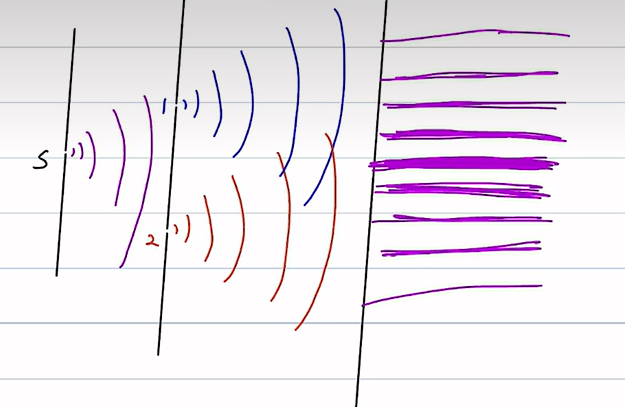
\includegraphics[width=0.7\linewidth]{figure/screenshot008}
\end{figure}

用$|s\rangle $标记通过缝s的态

用$|1\rangle $标记通过缝1的态

用$|2\rangle $标记通过缝2的态

用$|x\rangle $标记打到光屏$x$处的态

则通过缝$s$并且通过缝1的概率幅为$\left< 1 \middle| s \right>$

而通过缝1打到屏上$x$处的概率幅为$\left< x \middle| 1 \right>$

于是$s$发出的电子通过1打到屏上$x$处的概率幅为$\left< x \middle| 1 \right>$$\left< 1 \middle| s \right>$

同理$s$发出的电子通过2打到屏上$x$处的概率幅为$\left< x \middle| 2 \right>$$\left< 2 \middle| s \right>$

电子打到屏上x处的概率幅为
\begin{equation}
	\left< x \middle| s \right>	=\left< x \middle| 1 \right>\left< 1 \middle| s \right>+\left< x \middle| 2 \right>\left< 2 \middle| s \right>
\end{equation}

即
\begin{equation}
	\psi=c_1\psi_1+c_2\psi_2\quad\text{其中}|c_1|^2+|c_2|^2=1
\end{equation}

则$|c_1|^2$就是处于$\psi_1$的概率,$|c_2|^2$就是处于$\psi_2$的概率

这保证了波函数统计诠释的统一性

值得一提的是,若开三个缝,则$	\left< x \middle| s \right>	=\left< x \middle| 1 \right>\left< 1 \middle| s \right>+\left< x \middle| 2 \right>\left< 2 \middle| s \right>+\left< x \middle| 3 \right>\left< 3 \middle| s \right>$

即$\psi=c_1\psi_1+c_2\psi_2+c_3\psi_3$

若开n个缝,则$\left< x \middle| s \right>=\left< x \middle| s \right> =\sum_{i=1}^n{\left< x \middle| i \right> \left< i \middle| s \right>}
$

即$\psi=\sum_{i=1}^n{c_i\psi_i}$

甚至我们可以在双缝后面再开双缝
\begin{figure}[H]
	\centering
	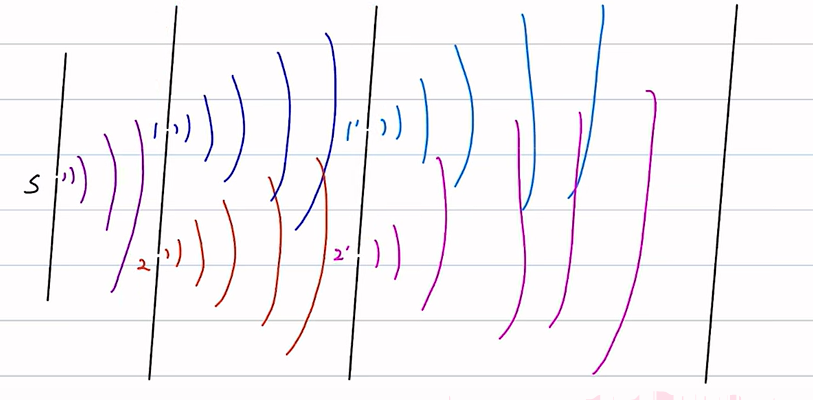
\includegraphics[width=0.7\linewidth]{figure/screenshot009}
\end{figure}

则最终达到接收屏上x处的概率振幅
\begin{equation}
	\begin{split}
		\left< x \middle| s \right> &=\left< x \middle| 1 '\right> \left< 1' \middle| 1 \right> \left< 1 \middle| s \right> +\left< x \middle| 1' \right> \left< 1' \middle| 2 \right> \left< 2 \middle| s \right> 
		\\
		&=\left< x \middle| 2 '\right> \left< 2' \middle| 1 \right> \left< 1 \middle| s \right> +\left< x \middle| 2' \right> \left< 2' \middle| 2 \right> \left< 2 \middle| s \right> 
	\end{split}
\end{equation}

若两个挡板都开n个缝
\begin{equation}
	\left< x \middle| s \right> =\sum_i^n{\sum_j^n{\langle x|i\rangle \langle i|j\rangle \langle i|s\rangle}}
\end{equation}

若m个挡板n个缝
\begin{equation}
	\left< x \middle| s \right> =\mathop {\underbrace{\sum_i^n{\sum_j^n{\sum_k^n{\cdots \sum_?^n{}}}}}} \limits_{m\text{个求和号}}\left< x \middle| i \right> \left< i \middle| j \right> \left< j \middle| \cdots \right> \cdots \left< \cdots \middle| ? \right> \left< ? \middle| s \right> 
\end{equation}

令m和n趋向于$\infty$,则我们就遍历了整个空间,这样我们就知道了自由空间中电子由s到单班x处的概率幅,它与s到屏上x处的所有可能路径有关、

\subsection{Bohr的氢原子模型}
\subsubsection{Bohr之前的原子模型}
a.J.J.Thompson的枣糕模型——被$\alpha$粒子散射实验否定
\begin{figure}[H]
	\centering
	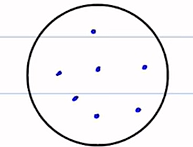
\includegraphics[width=0.7\linewidth]{figure/screenshot0010}
\end{figure}
1909年Rutherford和他的学生做了用$\alpha$粒子轰击铝箔的实验

\begin{figure}[H]
	\centering
	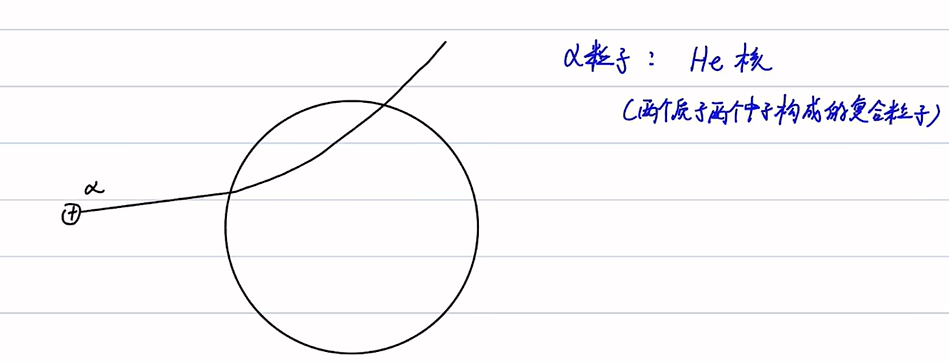
\includegraphics[width=0.7\linewidth]{figure/screenshot0011}
\end{figure}

\textbf{实验结果:}

绝大多数是小角度散射,但有$\dfrac{1}{8000}$的$\alpha$粒子偏转大于90°,甚至有180°原路返回的\textbf{(枣糕模型无法解释)}

b.Rutherford的行星轨道模型
\begin{figure}[H]
	\centering
	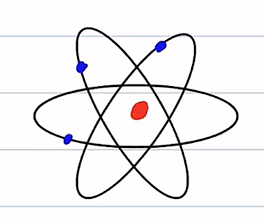
\includegraphics[width=0.7\linewidth]{figure/screenshot0012}
\end{figure}

原子中绝大部分区域都是空的?原子核带有原子绝大部分的质量和所有正电荷居于一个很小的区域,电子则像行星绕太阳一样绕着原子核公转

\begin{enumerate}
	\item 不能解释原子的稳定性
	\item 不能解释原子的分立光谱
\end{enumerate}
\subsubsection{氢原子光谱和Bohr原子模型}

\begin{figure}[H]
	\centering
	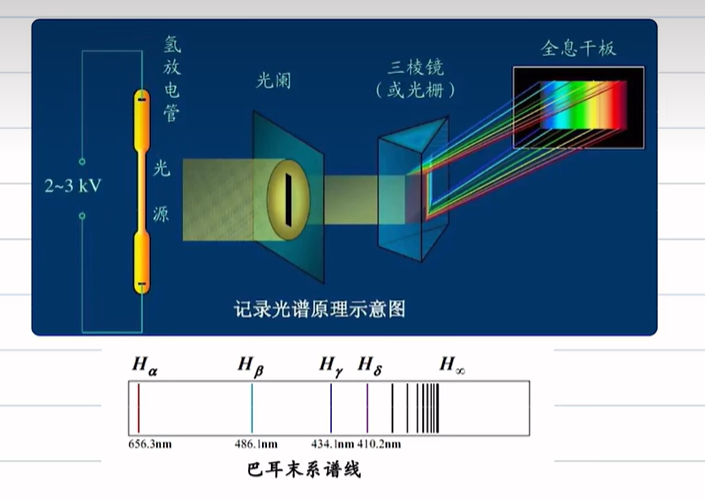
\includegraphics[width=0.7\linewidth]{figure/screenshot0014}
\end{figure}

实验给出氢原子的光谱为
\begin{equation}
	\tilde{v}\left( m,n \right) =R_H\left( \frac{1}{m^2}-\frac{1}{n^2} \right) =T\left( m \right) -T\left( n \right) 
\end{equation}

Bohr模型提出的基础(1913年)
\begin{enumerate}
	\item Rutherford行星轨道模型(部分继承)
	\item Plunk对黑体辐射理论的大胆创新(提出能量是分立的)以及Einstein对光电效应的解释和光子说($E=h$$\nu$)
	\item 氢原子光谱的经验公式
\end{enumerate}
Bohr模型的三大假设
1.核式模型+定态假设

电子运动在库仑力的作用下绕核做圆周运动

对于坍塌问题,$Bohr$则直接强行假定电子绕原子核做圆周运动时,只能处在一些分立的轨道上,并具有稳定的能量(定态假设)

2.辐射条件

当原子中的电子从一个定态n跃迁到另一个定态m时,会以电磁波的形式放出/吸收能量

3.角动量量子化

Bohr假设
\begin{equation}
	L=m_evr=n\frac{h}{2\pi}=n\hbar
\end{equation}
最终可得到
\begin{equation}
	E_n=-\frac{hcR_H}{n^2}=-hcT(n)
\end{equation}
于是
\begin{equation}
	h\nu_{m\rightarrow n}=E_n-E_m=hc(T(m)-T(n))
\end{equation}
其结论和氢原子谱线经验公式吻合地非常好

也得出$\nu_{m\rightarrow n}$=0,这与Bohr的定态假设是自洽的

成功之处
\begin{enumerate}
	\item 首次揭示了原子内部遵从量子规律,经典结论不再完全适用
	
	\item 成功解释了氢原子和类氢原子光谱
\end{enumerate}

不足之处
\begin{itemize}
	\item 半吊子的量子力学,提出量子化的概念,却又沿用经典力学中坐标、速度、轨道的概念
	\item 太强行
	\item 只适用于氢原子和类氢原子,完全处理不了多电子体系(没考虑电子间相互作用  )
\end{itemize}
\subsection{矩阵力学}

Heiseinberg几乎在同一时间以独立的方式给出了量子力学的另一种等价形式——矩阵力学

他主张:整个量子论只能从可观测量/力学量为基础,因此Bohr理论中的“轨道根本没有意义(不可观测)”

只有能极差才有价值,因为它是一个可观测量(频率谱线)

由于从一个状态到另一个状态的变化由两个状态(初,末)共同决定

而初,末状态分别由一系列数来决定

这两系数中的任何一个数都会影响可观测量

因此描述可观测量的应该是二维的

其元素数目应为$N_{\text{初}}\times N_{\text{末}} $,由于$N_{\text{初}}= N_{\text{末}} =N$,元素数目为$N^2$

于是Heiseinberg提出应用二维的数表(今天我们称之为矩阵)来表示状态的改变方式。

作为算符(operator),对应一种观测(操作)

用一维的数列(列矩阵)来表示状态

算符的作用是使一个态转换成另一个态

$\overset{\hat{O}}{\overbrace{\left[ \begin{matrix}
			&		&		\\
			&		&		\\
			&		&		\\
		\end{matrix} \right] }}\overset{\psi}{\overbrace{\left[ \begin{array}{c}
			\\
			\\
			\\
		\end{array} \right] }}=\overset{\psi'}{\overbrace{\left[ \begin{array}{c}
			\\
			\\
			\\
		\end{array} \right] }}$
	
	
可记为$\hat{O}|\psi \rangle =|\psi' \rangle $

\section{线性代数回顾}
\subsection{线性矢量空间}

\textbf{Definition1:}线性矢量空间$V$是由众多矢量$|v_i \rangle $构成的集合

矢量和:$|v_1 \rangle $+$|v_2 \rangle $

矢量数乘::$a|v \rangle $

其满足如下的运算法则(这个就是高代的线性空间的性质)
\begin{enumerate}
	\item 封闭性:矢量空间任意矢量的任意线性组合仍在矢量空间中
	\item 数乘的分配律:$a(|v_1 \rangle +|v_2 \rangle)=a|v_1 \rangle +a|v_2 \rangle$
	\item 矢量和的交换律:$|v_1 \rangle $+$|v_2 \rangle $=$|v_2 \rangle $+$|v_1 \rangle $
	\item 矢量和的结合律
	\item 零元素存在性
	\item 负元素存在性
\end{enumerate}

所有的2$\times$2矩阵是否构成线性空间?(满足)

所有定义在$(a,b) $上的函数是否构成?(满足)

这个看起来很反直觉,因为通常认为矢量具有大小和方向,大多数人对矢量的直观印象就是一个个的箭头,而矩阵和函数似乎并不满足人们对矢量的要求,但却是构成线性空间的,所以我们要抛弃对矢量空间的成见

\textbf{Definition2}:构造矢量空间$\mathbb{V}$时用到的所有可能的组合乘数$a$所在的空间称为$\mathbb{V}$的基域

若基域由所有实数组成,则称$\mathbb{V}$是一个实矢量空间

若基域由所有复数组成,则称$\mathbb{V}$是一个复矢量空间

\textbf{Definition3}:线性相关性

若一组矢量满足$\sum_{i=1}^n{a_i|v_i\rangle =|0\rangle}$有平凡解(所有的系数$a_i$都为0)则称他们时线性关的,若只有平凡解则称为是线性无关的

\textbf{Definition4}:若一个线性空间最多有n个线性无关的矢量,则称该线性空间是几维的

 \textbf{Definition5}:若$|v\rangle$是n维矢量空间中的矢量,则$|v\rangle$一定可以写成几个线性无关的矢量的线性组合
 
\textbf{Definition6}:n维度线性空间下的n个线性无关的矢量称为该线性空间的一组基()basis,一般来说不是唯一的

\textbf{Definition7}:矢量在基下的展开系数称为这组基下的分量(component)

\textbf{Definition8}:对于给定的基,同一矢量的分量是唯一的
\subsection{内积空间}

对于两个箭头形式的矢量点乘,我们有$\overrightarrow{A}\cdot \overrightarrow{B}=|\overrightarrow{A}|\cdot |\overrightarrow{B}|\cos \theta =\sum_{i=1}^n{a_ib_i}
$

其满足如下性质
\begin{enumerate}
	\item $\overrightarrow{A}\cdot \overrightarrow{B}=\overrightarrow{B}\cdot \overrightarrow{A}$
	\item $\overrightarrow{A}\cdot \overrightarrow{B}\ge 0$
	\item $\overrightarrow{A}\cdot \left( b\overrightarrow{B}+c\overrightarrow{C} \right) =b\overrightarrow{A}\cdot \overrightarrow{B}+c\overrightarrow{A}\cdot \overrightarrow{C}
	$
\end{enumerate}

我们希望抽象形式的矢量也满足同样的性质

\subsubsection{Dirac符号}
由于在给定基下矢量的各分量是唯一的$|v\rangle$=$\sum_{i}v_i|v_i\rangle$

因此,可以把矢量写成一个列矩阵

\begin{equation}
	|v\rangle =\left[ \begin{array}{c}
		v_1\\
		v_2\\
		v_3\\
		\vdots\\
		v_n\\
	\end{array} \right] \text{其中}n\text{是}LVS\text{的维度}
\end{equation}
其列矩阵的各分量即是$|v\rangle$在这组基下的各分量

我们把矢量$|A\rangle$和矢量$|B\rangle$的内积记为$\langle A|B\rangle $

因为我们希望内积是一个数,因此$\langle A|$是一个行矩阵

我们称$\langle |$为bra(左矢),其在一组基下的具体形式是一个行矩阵

$|\rangle$ket(右矢),其在一组基下的具体形式是一个列矩阵

内积应满足如下性质
\begin{itemize}
	\item $\langle V|V\rangle \ge 0$,矢量的模长是一个非负实数
	\item $\langle A|B\rangle $=$\langle B|A\rangle^* $在实矢量空间中退化为$\langle A|B\rangle $=$\langle B|A\rangle $,这保证了$\langle V|V\rangle $是实数
	\item $\langle A|B\rangle =\sum_{i}^{n}a^{*}_i b_i=\left[ \begin{matrix}
		a_{1}^{*}&		a_{2}^{*}&		a_{3}^{*}&		\cdots\\
	\end{matrix}\,\,a_{n}^{*} \right] \left[ \begin{array}{c}
		b_1\\
		b_2\\
		b_3\\
		\vdots\\
		b_n\\
	\end{array} \right] $
\end{itemize}

所以$\langle V|$在形式上是$|V\rangle$的转置共轭(又称厄米共轭),记作
\begin{equation}
	\left( |V\rangle \right) ^{\dagger}=\langle V|
\end{equation}

反过来亦然
\begin{equation}
	\left( \langle V| \right) ^{\dagger}=|V\rangle 
\end{equation}

与箭头形式的矢量内积相同的是,两个矢量内积模方的相对大小反映了两矢量的重叠程度

值得注意的是,左矢在线性性的地方$\langle aV|=a^*\langle  V|$

这就保证了$\langle aV|aV\rangle $是个实数

在此基础上,我们可以有

\textbf{Definition1}:满足所有内积性质的线性空间被称为内积空间

\textbf{Definition2}:若$\langle A|B\rangle $=0,则称这两个是正交的

\textbf{Definition3}:$\sqrt{\langle V|V\rangle }$称为$|V\rangle$的范数,若其范数唯一,则称$|V\rangle$为归一化的矢量

\textbf{Definition4}:一组范数均为1且两两正交的基称为正交归一基

对于一组线性无关基,总可以构造出一组正交归一的基,对于正交归一的基有
\begin{equation}
	\langle v_i|v_j\rangle =\delta _{ij}=\begin{cases}
		0,i\ne j\\
		1,i=j\\
	\end{cases}
\end{equation}
其中$\delta _{ij}$称为Kronecker delta符号

\subsection{正交归一基}
\subsubsection{矢量在一组正交归一基下的展开}
Q:已知一给定的矢量和一组正交归一基,如何确定其展开系数?
即\begin{equation*}
	|v\rangle=\sum_{i}v_i|v_i\rangle
\end{equation*}

A:两边同时左乘$\langle V|$
\begin{equation*}
	\begin{split}
		\langle v_j|v\rangle&=\sum_{i}v_i\langle v_j|v_i\rangle\\
		&=\sum_{i}v_j\delta_{ij}\\
		&=v_j
	\end{split}
\end{equation*}

于是我们可以将$|v\rangle$表示为$|v\rangle=\sum_{i}	\langle v_i|v\rangle|v_i\rangle$

由于$\langle v_i|v\rangle$是数,可以调换其位置,故
\begin{equation*}
	|v\rangle =\sum_i{|v_i\rangle \langle v_i|v\rangle}
\end{equation*}

因此$ |v\rangle =\sum_i|v_i\rangle \langle v_i|v\rangle$
	
另外,我们称$\hat{P}=|v_i\rangle \langle v_j|\text{为}|v_i\rangle \text{的投影算符}$

因为
\begin{equation*}
	\begin{split}
		\hat{P}|v\rangle &=\hat{P}\sum_i|v_i\rangle \langle v_i|v\rangle\\&=v_i|v_i\rangle
	\end{split}
\end{equation*}
它挑选了任意矢量$|v\rangle$中沿着$|v_i\rangle$的部分

用n个线性无关的基矢构成一组正交归一基的方法

\subsubsection{Schmidt正交化}
以三个线性无关的矢量为例$|1\rangle,|2\rangle,|3\rangle$

1.将$|1\rangle$放缩为$|I\rangle$,使$\langle I|I\rangle=1$

若$|2\rangle$与$|1\rangle$不正交,则$\langle 1|2\rangle\ne0$,即$|2\rangle$中有与$|1\rangle$平行的分量,其大小为$\langle 1|2\rangle$

2.将$|2\rangle$中与$|1\rangle$平行的分量减去

$|2'\rangle=|2\rangle-\langle 1|2\rangle|1\rangle$

再将$|2'\rangle$放缩为$|II\rangle$,使$\langle II|II\rangle=1$

3.将$|3\rangle$中与$|1\rangle$平行的分量和与$|2\rangle$平行的分量减去

$|3'\rangle=|3\rangle-\langle 1|3\rangle|1\rangle-\langle 2|3\rangle|2\rangle$

再将$|3'\rangle$放缩为$|III\rangle$,使$\langle III|III\rangle=1$

则$|I\rangle$,$|II\rangle$,$|III\rangle$为一组正交归一基
\subsection{线性算符}
算符的作用是使一个矢量变成另一个矢量

$\hat{O}|v\rangle =|v'\rangle$ 

$|v\rangle$和$|v'\rangle$都是n维的列矩阵

所以$\hat{O}$的具体形式是一个n$\times$n的方矩阵

我们只关心线性算符

矩阵一般是不对易的,即
\begin{equation*}
	\hat{O}\hat{\Omega}\ne \hat{\Omega}\hat{O}
\end{equation*}

我们称$\left[ \hat{O},\hat{\Omega} \right] =\hat{O}\hat{\Omega}-\hat{\Omega}\hat{O}
$为$\hat{O},\hat{\Omega}$的对易子

例:已知绕$Z$轴旋转90°的算符为$\hat{R}_Z=\left[ \begin{matrix}
	0&		-1&		0\\
	1&		0&		0\\
	0&		0&		1\\
\end{matrix} \right] $,绕x轴旋转90°的算符为$\hat{R}_X=\left[ \begin{matrix}
1&		0&		0\\
0&		0&		-1\\
0&		1&		0\\
\end{matrix} \right] $

他们是否对易?考察他们先后作用在$|\alpha\rangle=\left[ \begin{array}{c}
	a\\
	b\\
	c\\
\end{array} \right] $上的效果

$\hat{R}_Z\hat{R}_X=\left[ \begin{matrix}
	0&		0&		1\\
	1&		0&		0\\
	0&		1&		0\\
\end{matrix} \right] ,\hat{R}_X\hat{R}_Z=\left[ \begin{matrix}
	0&		-1&		0\\
	0&		0&		-1\\
	1&		0&		0\\
\end{matrix} \right] $

故不对易

现在我们考察$|\alpha \rangle \langle \beta |$

$\left[ \begin{array}{c}
	\alpha _1\\
	\alpha _2\\
	\vdots\\
	\alpha _n\\
\end{array} \right] \left[ \beta \begin{matrix}
	_{1}^{*}&		\beta _{2}^{*}&		\cdots&		\beta _{n}^{*}\\
\end{matrix} \right] $

故$|\alpha  \langle  |$是一个算符,这种运算称为矢量的外积

由矩阵乘法的转置,我们可推得$\left( \hat{A}\hat{B} \right) ^{\dagger}=\left( \left( \hat{A}\hat{B} \right) ^* \right) ^T=\hat{A}^{\dagger}\hat{B}^{\dagger}
$
\subsubsection{厄米算符$\&$反厄米算符}

厄米算符:$\hat{O}^{\dagger}=\hat{O},\text{即}O_{ij}={O_{ji}}^*
$

反厄米算符:$\hat{O}^{\dagger}=-\hat{O},\text{即}O_{ij}=-{O_{ji}}^*$

定理:任意算符都可以写成厄米算符和反厄密算符的线性组合(类比任何矩阵都可以写成对称矩阵和反对称矩阵的和)
\subsubsection{幺正算符}

\begin{equation*}
	\hat{U}^{\dagger}\hat{U}=\hat{I}
\end{equation*}
通过幺正算符进行的线性变换称为幺正变换,其是保内积的

故其是一种抽象的旋转操作
\subsection{本征值和本征矢量}

若算符$\hat{O}$作用在某一矢量上的结果等价于将该矢量放缩一个倍数,则称该矢量为$\hat{O}$的本征矢量,该倍数称为$\hat{O}$的本征值
\begin{equation*}
	\hat{O}|n\rangle =O_n|n\rangle \,\,\text{称为}\hat{O}\text{的本征方程}
\end{equation*}

这个方程可能有不同的解,但注意$|n\rangle $和$|n\rangle $的任意倍数被视为同一个解

现在我们来讨论$\hat{O}$的本征值的具体求法
\begin{equation*}
	(\hat{O}-O_n)|n\rangle=|0\rangle
\end{equation*}
将$O_n$乘以一个单位矩阵1
\begin{equation*}
	(\hat{O}-O_n1)|n\rangle=|0\rangle
\end{equation*}

这是个$n$个方程$n$个未知数齐次线性方程组

其有非零解的条件是其系数行列式为0
\begin{equation*}
	\rightarrow|	(\hat{O}-O_n)|=0
\end{equation*}

通过这个方程我们就能解出本征值$O_n$,再将$O_n$代入本征方程即可解出本征矢

有时候,同一本征值会对应多个本征矢,这种情况叫做简并

定理二:对应厄米算符不同本征值的本征矢量相互正交

定理三:幺正算符的本征值是模长为1的复数

\subsubsection{厄米算符的对角化}
定理1:算符在用其自身一组正交归一本征矢构成的的基下表示为一个对角矩阵

定理2:若$\hat{O}$在某正交归一基下是一个Hermite矩阵,则总存在一个幺正矩阵$\hat{U}
$使得$\hat{U}^{\dagger}\hat{O}\hat{U}$在该基下是对角矩阵

以上的证明为高代内容,参考高代笔记

\chapter{理论基础}
\section{Stem-Granch实验}
\begin{figure}[H]
	\centering
	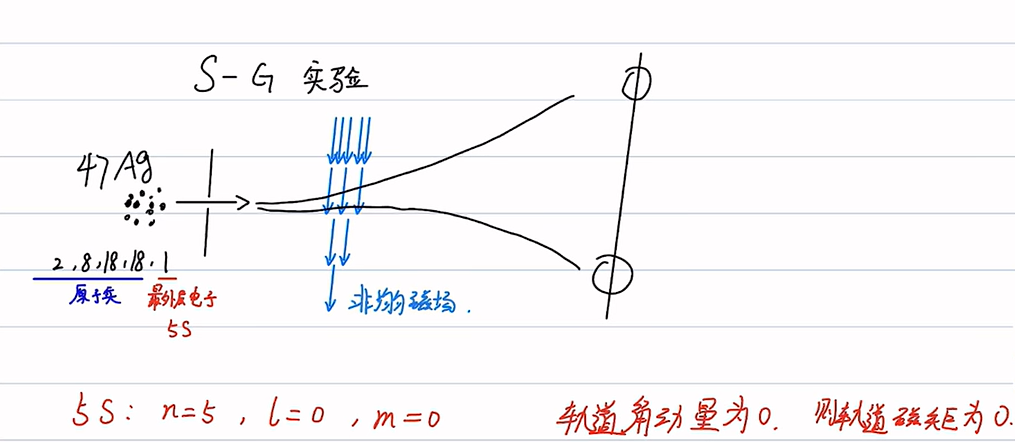
\includegraphics[width=0.9\linewidth]{figure/screenshot0015}
\end{figure}
磁矩在非均匀磁场中z方向的受力$F_z=\mu\frac{\partial B_z}{\partial z}$

但银原子束分裂了,且分裂成独立的两束

which tells us

I.电子除轨道角动量还有某个“角动量”

II.这个角动量的大小为$\frac{1}{2}\hbar$

1925年Uhlenbeck和Goudsimt提出电子有自选假设:

(1)每一个电子都具有内禀角动量(自旋角动量)$\hat{S}$,其大小为$\frac{1}{2}\hbar$

(2)自旋磁矩与自旋角动量的关系:
$\begin{cases}
	\widehat{\mu }_s=-\frac{e}{2m_e}g_s\hat{S}\,\,\quad \left( \text{轨道磁矩} \widehat{\mu }_l=-\frac{e}{2m_e}g_l\hat{L} \right)\\
	g_s=2\quad  \left( g_l=1 \right)\\
\end{cases}$

因此我们效仿杨氏双缝,将向上偏转的电子态记为$|\uparrow \rangle $,向下偏转的电子态记为$\downarrow$

\subsection{级联S-G实验}
\begin{figure}[H]
	\centering
	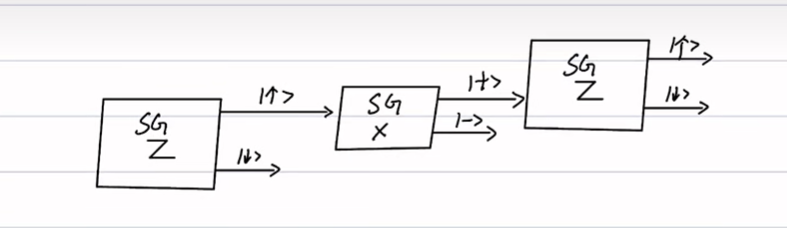
\includegraphics[width=0.7\linewidth]{figure/screenshot0016}
\end{figure}

银原子未通过z方向的SG后分裂成两束,一束向上偏移,一束向下偏移

取自旋态$|\uparrow \rangle $的粒子来通过x方向的SG装置,结果一束向x正方向偏转,一束向x负方向偏转,分别占总数的50$\%$

再取x正方向($|+ \rangle $)的粒子束通过第二个z方向的SG装置

结果还是一束向上偏移,一束向下偏移

这个结果很反直觉,因为我们再第一步就已经把z方向自旋向上的粒子挑选出来了

\begin{enumerate}
	\item  这个实验说明,对于$S_x$的测量把粒子$S_z$的信息抹去了,因此我们无法同时得到粒子$S_z$和$S_x$的信息,我们称$S_z$和$S_x$是互不相容的可观测量
	\item  $|\uparrow \rangle $包含了$|+ \rangle $和$|- \rangle $的成分,各占一半,$|+ \rangle $包含了$|\uparrow \rangle $和$|\downarrow \rangle $的成分,也各占一半
\end{enumerate}
这似乎告诉我们,在经典和量子世界中,测量扮演着十分不同的角色

\section{用线性代数的语言来描述力}
1、我们发现量子力学与线性代数有很多相似之处

\begin{enumerate}
	\item 可观测量在其本征态上有确定的值,矩阵作用在本征矢上得到一个确定的值
	\item 叠加态原理告诉我们不同的态可以线性叠加成为一个新的可能态,矢量之间也可以通过线性叠加构造一个新的矢量
	\item S.eq是线性偏微分方程,其同解为本征解(特解)的线性组合,这些本征解可以作为LVS的基,任意的通解可以通过基前面的系数的组合来表述
	\item 可观测量由初,末两个状态来决定,应是二维的,而测量会使一个态转化为另一个态,矩阵是二阶张量,矩阵作用在一个矢量上会使其变为另一个矢量
\end{enumerate}
因此,我们可以用矢量来描述量子系统的状态(称为态矢量),

$|\psi \rangle $:态矢量,它包含了系统的全部信息

$|\hat{O} \rangle $:力学量

但并不是所有的矩阵都能描述力学量

因为可观测量是物理的,即其测量值(本征值)应为实数,因此其应用一个厄米矩阵来描述
\subsection{拓展到无穷维}

量子力学体系中,很多系统无法用有限个维度来描述,而是无穷维的,这个时候我们能就要对我们在第一章所学的线代知识经行拓展

考虑定义在$[a,b]$上的函数$f(x)$
\begin{figure}[H]
	\centering
	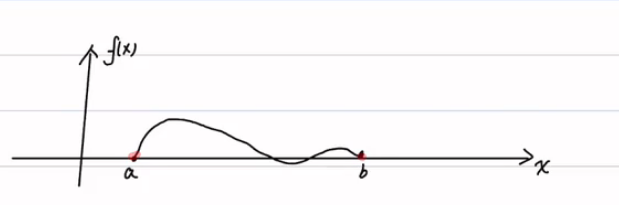
\includegraphics[width=0.7\linewidth]{figure/screenshot0017}
\end{figure}


要用到一个列向量来描述这一函数,只需要用每处$x_i$的函数值$f(x_i)$作为矩阵元素构造,将$a-b$分为n等份
\begin{equation*}
	|f\rangle =\left[ \begin{array}{c}
		f\left( x_1 \right)\\
		f\left( x_2 \right)\\
		\vdots\\
		f\left( x_n \right)\\
	\end{array} \right] \text{即}f\text{在每一}x_i\text{的函数值等于}|f\rangle \text{用}|x_i\rangle \text{展开的展开系数}
\end{equation*}

而该空间生成的基矢为$|x_i\rangle=|x_i\rangle =\left[ \begin{array}{c}
	0\\
	0\\
	\vdots\\
	\mathop 1 \limits_{\text{第}i\text{个位置}}\\
	\vdots\\
	0\\
\end{array} \right]$

则$|x_i\rangle$所有的线性组合构成的矢量构成一个LVS,其维度为n,当n趋近于$\infty$时构成了无穷维LVS
\subsection{内积}

若沿用离散有限维时的内积定义
\begin{equation*}
	\langle f|g\rangle =\underset{n\rightarrow \infty}{\lim}\sum_i^n{f^*\left( x_i \right) g\left( x_i \right)}
\end{equation*}

由于$f^*\left( x_i \right) g\left( x_i \right)$都是有限的,因此求和可能会无限大

这样我们需要对无限维的内积重新进行定义

一个合乎情理的方式是,取其在每个点上的平均值,这样结果一定是有界的,故
\begin{equation*}
	\begin{split}
		\langle f|g\rangle &=\underset{n\rightarrow \infty}{\lim}\sum_i^n{f^*\left( x_i \right) g\left( x_i \right)}\frac{1}{n+1}
		\\
		&=\int\limits_a^b{f^*\left( x_i \right) g\left( x_i \right) dx}
	\end{split}
\end{equation*}

由于$\left. \begin{array}{r}
	f\left( x \right) =\langle x|f\rangle\\
	g\left( x \right) =\langle x|g\rangle\\
\end{array} \right\} \rightarrow f^*\left( x \right) =\langle f|x\rangle 
$

因此
\begin{equation*}
	\begin{split}
		\langle f|g\rangle &=\int\limits_a^b{f^*\left( x_i \right) g\left( x_i \right) dx}
		\\
		&=\int\limits_a^b{\langle f|x\rangle \langle x|g\rangle dx}	
	\end{split}
\end{equation*}

得到$\int\limits_a^b{| x\rangle \langle x| dx}=1	$
\subsection{Dirac归一化}

我们考虑连续空间中基矢的正交归一性

由于这个无穷维的矢量空间中的个基矢不含彼此的成分

因此$\langle x|x'\rangle$=0$x\ne x'$

但$\langle x|x'\rangle$在$x=x'$时也是否为1则是个未知数,内积定义变了

将$|f\rangle$用$|x'\rangle$展开
\begin{equation*}
	|f\rangle =\int\limits_a^b{|x'\rangle \langle x'|f\rangle dx'}
\end{equation*}

两边同时左乘$\langle x|$
\begin{equation*}
	f(x)=\langle x|f\rangle =\int\limits_a^b{\langle x|x\rangle \langle x|f\rangle dx}
\end{equation*}

由于此$\langle x|x'\rangle$在x$\ne$x'处全为零

因此积分区间可改写为$ x$附近的无穷小邻域
\begin{equation*}
	\begin{split}
		f\left( x \right) &=\int\limits_{x-\varepsilon}^{x+\varepsilon}{\langle x|x\rangle \langle x'|f\rangle dx'}
		\\
		&=f\left( x \right) \int\limits_{x-\varepsilon}^{x+\varepsilon}{\langle x|x'\rangle dx'}
		\\
		&\rightarrow \int\limits_{x-\varepsilon}^{x+\varepsilon}{\langle x|x'\rangle dx'}=1
	\end{split}
\end{equation*}
要在无穷小区间上积分为有限值,则$\langle x|x'\rangle$在积分区间上不能是有限值

则$\langle x|x\rangle=\infty,x\in[x-\varepsilon,x+\varepsilon]$

因此$\langle x|x'\rangle$应该满足这样的性质
\begin{equation*}
	\begin{cases}
		\langle x|x'\rangle =0,x\ne x'\\
		\langle x|x'\rangle =\infty ,x=x'\\
	\end{cases}
\end{equation*}

为了方便起见,我们定义一一个新的函数$\langle x|x'\rangle=\delta(x-x') $,其满足
\begin{equation*}
	\delta \left( x-x' \right) =\begin{cases}
		0,x\ne x'\\
		\infty ,x=x'\\
	\end{cases}.\int_{-\infty}^{+\infty}{\delta \left( x-x' \right)}=1
\end{equation*}
 
 其图像一般表示为:
 \begin{figure}[H]
 	\centering
 	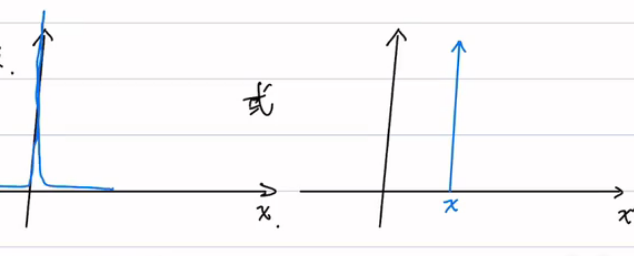
\includegraphics[width=0.7\linewidth]{figure/screenshot0018}
 \end{figure}
 显然其为关于x的偶函数
 \subsubsection{Dirac-$\delta$函数的性质}
 \begin{enumerate}
 	\item 采样性:$\int_{-\infty}^{+\infty}{\delta \left( x-x' \right) f\left( x \right) dx}=f\left( x' \right) 
 	$
 	\item 放缩性:$\delta \left( ax \right) =\frac{1}{|a|}\delta \left( x \right) 
 	$
 	\item 实值性
 	\item $\delta$函数的傅里叶变换:
 	\begin{equation*}
 		\frac{1}{\sqrt{2\pi}}\int\limits_{-\infty}^{+\infty}{e^{-ikx}\delta \left( x-x' \right) dx=}\frac{1}{\sqrt{2\pi}}e^{-ikx'}
 	\end{equation*}
 	\item 含$\delta$函数的导数积分
 	\begin{equation*}
 	\delta' \left( x-x' \right) =\delta \left( x-x' \right) \frac{d}{dx}
 	\end{equation*}
 	\item 单位界越函数和$\delta$函数
 	\begin{figure}[H]
 		\centering
 		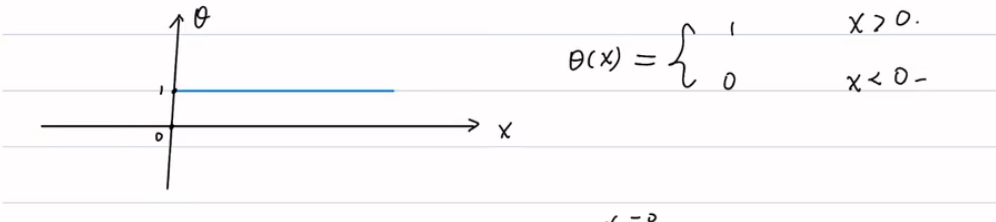
\includegraphics[width=0.7\linewidth]{figure/screenshot0019}
 	\end{figure}
 	\begin{equation*}
 		\frac{d}{dx}\theta =\begin{cases}
 			\infty ,x=0\\
 			0,x\ne 0\\
 		\end{cases}=\delta \left( x \right)\\
 	\end{equation*}
 \end{enumerate}
 \subsection{无穷维下的算符}
 无穷维下的右矢对应一个连续函数,因此无穷维的算符就是将一个函数$f(x)$变成另一个函数$\hat{f}(x)$
 \begin{equation*}
 	\hat{O}|f\rangle=|\hat{f}\rangle
 \end{equation*}
 
 最简单的例子便是\textbf{求导算}符$\hat{D}$
 \begin{equation*}
 		\hat{D}|f\rangle=|\frac{d}{dx}f\rangle
 \end{equation*}
 
 其中$|\frac{d}{dx}f\rangle$表示对应函数$f'(x)$的右矢,其每一个分量为$\frac{df}{dx}$即$f'(x)$
 
 那么$\hat{D}$在基$|x\rangle$下的矩阵表示是什么?
 
 这等价于求矩阵元
 在上式左乘$\langle x|$
 
 $\langle x|\hat{D}f|\rangle=\langle x|\frac{d}{dx}f\rangle=f'(x)$
 
 $\int{\langle x|\hat{D}|x'\rangle \langle x'|f\rangle dx' =f'(x)}$
 
 $\int{\hat{D}_{xx'}f\left( x' \right) dx'=f\prime(x)}$
 
 因此$\hat{D}_{xx'}=\delta'(x-x')$
 
 求导算符是反厄米算符: $\bar{D}^\dagger=-\bar{D}$
 
 \subsubsection{位置算符$\bar{X}$}
 $\bar{X}|x_j\rangle=x_j|x_j\rangle$
 $\rightarrow X_{ij}=x_j\delta(x_i-x_j)$
 
 因此$\bar{X}$在$|x\rangle$基下的矩阵表示为对角矩阵
 \subsubsection{无限维下的厄米算符}
 厄米算符是量子力学种我们特别关心的一类算符,因为厄米算符的本征值为实数,而可观测量是物理的,即测量到的结果(本征值)必须是实数,因此我们用厄米算符来表示可观测量
 
 命题:若$\bar{K}$为厄米算符,则$\langle \hat{K}f|g\rangle =\langle f|\hat{K}g\rangle  $
 
 这是说明$\bar{K}$为厄米算符的另一种判据,在不方便求解$\bar{K}^T$时十分有用
 \subsubsection{力学量的平均值}
 
 以位置为例,我们知道$|\psi(x)|^2$表示粒子在x处出现的概率密度,则x在全空间上的均值应等于$\int_{-\infty}^{+\infty}x\rho(x)dx$
 
 \begin{equation*}
 	\begin{split}
 		\bar{x}&=\int\limits_{-\infty}^{+\infty}{x\rho \left( x \right) dx}
 		\\
 		&=\int\limits_{-\infty}^{+\infty}{x|\psi \left( x \right) |^2dx}
 		\\
 		&=\int\limits_{-\infty}^{+\infty}{x\psi ^*\left( x \right) \psi \left( x \right) dx}
 		\\
 		&=\int\limits_{-\infty}^{+\infty}{\psi ^*\left( x \right) x\psi \left( x \right) dx}
 		\\
 		&=\langle \psi |x|\psi \rangle \text{记作}<x>
 	\end{split}
 \end{equation*}
 
 实际上,对于任意力学量$\bar{\Omega}$
 
 在$|\psi\rangle$态下对其测量时总是会落入对应特定本征值$\omega_i$的本征态$|\omega_i\rangle$
 
 而对应的概率为$P_i =|\langle\omega_i|\psi\rangle|^2$
 
 力学量<$\bar{\Omega}$>在某个态$|\psi\rangle$下的平均值为$\langle\psi|\bar{\Omega}|\psi\rangle$,\text{记作}<$\bar{\Omega}$>
 
 例:求自由粒子速度的平均值
 \begin{equation*}
 	\begin{split}
 		\bar{v}&=\frac{d\bar{x}}{dt}
 		\\
 		&=\frac{d}{dt}\int_{-\infty}^{+\infty}{x|\psi |^2}dx
 		\\
 		&=\int_{-\infty}^{+\infty}{\left( \frac{\partial}{\partial t}x|\psi |^2+x\frac{\partial}{\partial t}|\psi |^2 \right)}dx
 		\\
 		&=\int_{-\infty}^{+\infty}{x\frac{\partial}{\partial t}|\psi |^2}dx
 		\\
 		&=\int_{-\infty}^{+\infty}{x\frac{\partial}{\partial t}\psi ^*\psi}dx
 		\\
 		&=\int_{-\infty}^{+\infty}{x\left( \frac{\partial}{\partial t}\psi ^*\psi +\psi ^*\frac{\partial}{\partial t}\psi \right)}dx,\text{又}i\hbar \frac{\partial}{\partial t}\psi =\hat{H}\psi 
 		\\
 		&=\int_{-\infty}^{+\infty}{x\left( \frac{i}{\hbar}\hat{H}\psi ^*\psi -\psi ^*\frac{i}{\hbar}\hat{H}\psi \right)}dx
 		\\
 		&=\int_{-\infty}^{+\infty}{x\frac{i}{\hbar}\left( \hat{H}\psi ^*\psi -\psi ^*\hat{H}\psi \right)}dx
 		\\
 		&=\int_{-\infty}^{+\infty}{x\frac{i}{\hbar}\frac{\hbar ^2}{2\mu}\left( H\psi ^*\frac{\partial ^2}{\partial x^2}\psi -\frac{\partial ^2}{\partial x^2}\psi ^*\psi \right)}dx
 		\\
 		&=\int_{-\infty}^{+\infty}{x\frac{i}{\hbar}\frac{\hbar ^2}{2\mu}\frac{\partial}{\partial x}\left( \psi ^*\frac{\partial}{\partial x}\psi -\frac{\partial}{\partial x}\psi ^*\psi \right)}dx
 		\\
 		&=\frac{-ih}{2\mu}\left( \int_{-\infty}^{+\infty}{\psi ^*\frac{\partial}{\partial x}\psi dx-\int_{-\infty}^{+\infty}{d\psi ^*\psi}} \right) 
 		\\
 		&=\int_{-\infty}^{+\infty}{\psi ^*\frac{-ih}{\mu}\frac{\partial}{\partial x}\psi}dx
 		\\
 		&=\langle \psi |\frac{-ih}{\mu}\frac{\partial}{\partial x}|\psi \rangle =\left< v_x \right> 
 	\end{split}
 \end{equation*}
 
 \subsubsection{量子力学五大假设}
 \begin{enumerate}
 	\item 态假设:粒子的状态由Hilbert空间中的态矢量完备描述
 	\item 力学量假设:力学量由厄米算符描述
 	\item 测量假设:在$|\psi\rangle$态中对力学量$\hat{\Omega}$进行测量,会得到其本征值$\omega_i$,相应的概率为$ |\langle\omega_i|\psi\rangle|^2$,其中$|\omega_i\rangle$为$\omega_i$所对应的本征态
 	\item 演化假设:态的演化服从薛定谔方程
 	\item 全同粒子假设:内禀属性完全相同的粒子不可分辨
 	
 \end{enumerate}
 \section{自旋$\frac{1}{2}$系统的矩阵形式}
 
 1.在$\hat{S_z}$自身的本征矢构成的基下,$\hat{S_z}$是一个对角矩阵,其对角线元素即为本征值,因此

 取\begin{equation*}
 	|\uparrow \rangle =\left[ \begin{array}{c}
 		1\\
 		0\\
 	\end{array} \right] ,|\downarrow \rangle =\left[ \begin{array}{c}
 		0\\
 		1\\
 	\end{array} \right] 
 \end{equation*}
 则\begin{equation*}
 	\begin{split}
 		\hat{S}_z&=\left[ \begin{matrix}
 			\frac{\hbar}{2}&		0\\
 			0&		-\frac{\hbar}{2}\\
 		\end{matrix} \right] 
 		\\
 		&=\frac{\hbar}{2}|\uparrow \rangle \langle \downarrow |+\left( -\frac{\hbar}{2} \right) |\downarrow \rangle \langle \downarrow |
 	\end{split}
 \end{equation*}
 
 那在$\hat{S_2}$的矩阵形式是什么?(把在$\hat{S_z}$的上下换成正负即可)
 
 2.现在,问题在于,如何在$S_z $表象(以上下箭头为本征向量的)中表示$S_x $的矩阵
 
 波函数整体的相因子没有物理意义
 \begin{equation*}
 	\begin{split}
 		\rho =|\psi \left( x \right) |^2&=\psi ^*\left( x \right) \psi \left( x \right) 
 		\\
 		&=\psi \left( x \right) e^{-i\alpha}\psi \left( x \right) e^{i\alpha}
 		\\
 		&=|\psi \left( x \right) e^{i\alpha}|^2
 	\end{split}
 \end{equation*}
 同样,态矢量整体的相因子也没有物理意义
 
 则在级联S-G实验中
 \begin{equation*}
 	\begin{split}
 		|\uparrow \rangle &=\frac{1}{\sqrt{2}}e^{i\theta}|+\rangle +\frac{1}{\sqrt{2}}e^{i\varphi}|-\rangle ,\text{乘以一整体相因子物理意义不变}
 		\\
 		&=\frac{1}{\sqrt{2}}|+\rangle +\frac{1}{\sqrt{2}}e^{i\left( \varphi -\theta \right)}|-\rangle ,\text{令}\varphi -\theta =\delta _1
 		\\
 		&=\frac{1}{\sqrt{2}}|+\rangle +\frac{1}{\sqrt{2}}e^{i\delta _1}|-\rangle 
 	\end{split}
 \end{equation*}
 
 同理
 \begin{equation*}
 	\begin{split}
 		|+\rangle &=\frac{1}{\sqrt{2}}|\uparrow \rangle +\frac{1}{\sqrt{2}}e^{i\delta _2}|\downarrow \rangle 
 		\\
 		|-\rangle &=\frac{1}{\sqrt{2}}|\uparrow \rangle +\frac{1}{\sqrt{2}}e^{i\delta' _2}|\downarrow \rangle 
 	\end{split}
 \end{equation*}
 
 而$\langle -|+\rangle$=0,则
 \begin{equation*}
 	\left( \frac{1}{\sqrt{2}}|\uparrow \rangle +\frac{1}{\sqrt{2}}e^{i\delta _2}|\downarrow \rangle \right) \left( \frac{1}{\sqrt{2}}|\uparrow \rangle +\frac{1}{\sqrt{2}}e^{i\delta' _2}|\downarrow \rangle \right) =\frac{1}{2}+\frac{1}{2}e^{i\left( \delta _2-\delta' _2 \right)}=0
 \end{equation*}
 
 则$\frac{1}{2}e^{i\left( \delta _2-\delta' _2 \right)}=-1$
 
 即$\frac{1}{2}e^{i\left( \delta _2 \right)}=-\frac{1}{2}e^{i\left( \delta' _2 \right)}$
 
 于是
 \begin{equation*}
 	|-\rangle =\frac{1}{\sqrt{2}}|\uparrow \rangle -\frac{1}{\sqrt{2}}e^{i\delta _2}|\downarrow \rangle
 \end{equation*}
 
 则\begin{equation*}
 	\begin{split}
 		|+\rangle \langle +|&=\left( \frac{1}{\sqrt{2}}|\uparrow \rangle +\frac{1}{\sqrt{2}}e^{i\delta _2}|\downarrow \rangle \right) \left( \frac{1}{\sqrt{2}}|\uparrow \rangle +\frac{1}{\sqrt{2}}e^{i\delta _2}|\downarrow \rangle \right) 
 		\\
 		&=\frac{1}{2}\left( |\uparrow \rangle \langle \uparrow |+e^{-i\delta _2}|\uparrow \rangle \langle \downarrow |+e^{i\delta _2}|\downarrow \rangle \langle \uparrow |+|\downarrow \rangle \langle \downarrow | \right) 
 	\end{split}
 \end{equation*}
 
 \begin{equation*}
 	\begin{split}
 		|-\rangle \langle -|&=\left( \frac{1}{\sqrt{2}}|\uparrow \rangle -\frac{1}{\sqrt{2}}e^{i\delta _2}|\downarrow \rangle \right) \left( \frac{1}{\sqrt{2}}|\uparrow \rangle -\frac{1}{\sqrt{2}}e^{i\delta _2}|\downarrow \rangle \right) 
 		\\
 		&=\frac{1}{2}\left( |\uparrow \rangle \langle \uparrow |-e^{-i\delta _2}|\uparrow \rangle \langle \downarrow |-e^{i\delta _2}|\downarrow \rangle \langle \uparrow |+|\downarrow \rangle \langle \downarrow | \right) 
 	\end{split}
 \end{equation*}
 
 于是
 \begin{equation*}
 	\begin{split}
 		\hat{S}_x&=\frac{\hbar}{2}|+\rangle \langle +|-\frac{\hbar}{2}|-\rangle \langle -|
 		\\
 		&=\frac{\hbar}{2}\left( |\uparrow \rangle \langle \uparrow |+e^{-i\delta _2}|\uparrow \rangle \langle \downarrow |+e^{i\delta _2}|\downarrow \rangle \langle \uparrow |+|\downarrow \rangle \langle \downarrow | \right)\\ &-\frac{\hbar}{2}\left( |\uparrow \rangle \langle \uparrow |-e^{-i\delta _2}|\uparrow \rangle \langle \downarrow |-e^{i\delta _2}|\downarrow \rangle \langle \uparrow |+|\downarrow \rangle \langle \downarrow | \right) 
 		\\
 		&=\frac{\hbar}{2}\left( e^{-i\delta _2}|\uparrow \rangle \langle \downarrow |+e^{i\delta _2}|\downarrow \rangle \langle \uparrow | \right) ,\text{现选取}\hat{S}_z\text{表象}
 		\\
 		&=\frac{\hbar}{2}\left[ \begin{matrix}
 			0&		e^{-i\delta _2}\\
 			e^{i\delta _2}&		0\\
 		\end{matrix} \right] 
 	\end{split}
 \end{equation*}
 
 如何确定$\delta_2$?
 
 在此之前,我们要先考虑一下$\hat{S_y}$在$\hat{S_z}$表象中的形式,这个其实是一样的,因为用的条件一模一样
  \begin{equation*}
 	\begin{split}
 		|S_y+\rangle &=\frac{1}{\sqrt{2}}|\uparrow \rangle +\frac{1}{\sqrt{2}}e^{i\delta _3}|\downarrow \rangle 
 		\\
 		|S_y-\rangle &=\frac{1}{\sqrt{2}}|\uparrow \rangle -\frac{1}{\sqrt{2}}e^{i\delta _3}|\downarrow \rangle 
 	\end{split}
 \end{equation*}
 由于y是第三个轴,我们要对其加以约束
 \begin{equation*}
 	|<S_{y+1}|->|^{2}=|<S_{y-1}|->|^{2}= |<S_{y+1}|+>|^{2}= |<S_{y-1}|+>|^{2}=\frac{1}{2}
 \end{equation*}
 
 代入计算可得到
 \begin{equation*}
 	|1\pm e^{i\left( \delta _2-\delta _3 \right)}|^2=2
 \end{equation*}
 
$ \delta _2-\delta _3$只能为$\pm \frac{\pi}{2}$

$
\text{若选择}\delta _2-\delta _3=-\frac{\pi}{2}\text{则称我们所构建的坐标系为右手系}
\\
\text{若选择}\delta _2-\delta _3=\frac{\pi}{2}\text{则称我们所构建的坐标系为左手系}$

这里我们选取右手系,并选择$\delta_2=0,\delta_3=\frac{\pi}{2}$,带入数值,计算可算得

\begin{equation*}
	\begin{split}
		\hat{S}_x\hat{S}_z-\hat{S}_z\hat{S}_x&=\frac{\hbar ^2}{4}\left[ \begin{matrix}
			0&		1\\
			1&		0\\
		\end{matrix} \right] \left[ \begin{matrix}
			1&		0\\
			0&		-1\\
		\end{matrix} \right] -\frac{\hbar ^2}{4}\left[ \begin{matrix}
			1&		0\\
			0&		-1\\
		\end{matrix} \right] \left[ \begin{matrix}
			0&		1\\
			1&		0\\
		\end{matrix} \right] 
		\\
		&=\frac{\hbar ^2}{4}\left( \left[ \begin{matrix}
			0&		-1\\
			1&		0\\
		\end{matrix} \right] -\left[ \begin{matrix}
			0&		1\\
			-1&		0\\
		\end{matrix} \right] \right) 
		\\
		&=-i\hbar \hat{S}_y
	\end{split}
\end{equation*}
通过重复相同的计算,我们可以得到
\begin{equation*}
	[\hat{S}_{\alpha},\hat{S}_{\beta}]=\varepsilon _{\alpha \beta \gamma}i\hbar \hat{S}_{\gamma}
\end{equation*}
$\varepsilon_{\alpha\beta\gamma}$称为levu-civita记号,逆序数为偶数时等于1,逆序数为奇时为-1


还可以定义
\begin{equation*}
	\begin{split}
		\hat{S}^2&={\hat{S}_x}^2+{\hat{S}_y}^2+{\hat{S}_z}^2
		\\
		&=\frac{3}{4}\hbar ^2
	\end{split}
\end{equation*}
\subsection{(不)相容力学量和对易关系}

在级联S-G实验中,我们可以看到,$\hat{S}_{x}$的取值和$\hat{S}_{z}$的取值是无法被同时确定的,这也很显然,因为力学量只在其本征态下在取确定的值

而$\hat{S}_{z}$的本征态对于$\hat{S}_{x}$来说是叠加态(反之亦然)
 \begin{equation*}
	\begin{split}
		|+\rangle &=\frac{1}{\sqrt{2}}|\uparrow \rangle +\frac{1}{\sqrt{2}}|\downarrow \rangle 
		\\
		|-\rangle &=\frac{1}{\sqrt{2}}|\uparrow \rangle +\frac{1}{\sqrt{2}}|\downarrow \rangle 
	\end{split}
\end{equation*}

我们称这样的,一个力学量$\hat{A}$对于另一个力学量$\hat{B}$而言是叠加态(从而$\hat{A}$,$\hat{B}$无法同时取到确定的值)的力学量为\textbf{不相容力学量}

那么.有没有这样一种情况,力学量$\hat{A}$和力学量$\hat{B}$存在一组共同的本征态,这样$\hat{A}$,$\hat{B}$就可以同时取确定的值了呢?

答案是可以的.我们称这样的力学量为相容力学量

因为算符对应着测量,因此如果$\hat{A}$和$\hat{B}$可以同时取确定的值,则先测$\hat{A}$后测$\hat{B}$还是先测$\hat{B}$后测$\hat{A}$应没有区别,则$\hat{A}$$\hat{B}$=$\hat{B}$$\hat{A}$,即[$\hat{A}$,$\hat{B}$]=0

所以我们断言,$\text{力学量}\hat{A}\text{和}\hat{B}\text{存在一组共同的本征态}\Leftrightarrow \left[ \hat{A},\hat{B} \right] =0$


思考题:

1.若$\left[ \hat{A},\hat{B} \right] =0$,则$\hat{A}$的所有本征态都必定是$\hat{B}$的本征态?错,只能说明有一组本征态相同

2.若$\left[ \hat{A},\hat{B} \right] =0$,$\left[ \hat{A},\hat{C} \right] =0$,则$\left[ \hat{C},\hat{B} \right] =0$?错,本征态不一定相同



计算$[x,\hat{P_x}$

将其作用在任意波函数上
\begin{equation*}
	\begin{split}
		\left[ x,\hat{P}_x \right] \psi \left( x \right) &=x\hat{P}_x\psi \left( x \right) -\hat{P}_xx\psi \left( x \right) 
		\\
		&=-i\hbar \left( x\frac{d}{dx}\psi \left( x \right) -\psi \left( x \right) -x\frac{d}{dx}\psi \left( x \right) \right) 
		\\
		&=i\hbar \psi \left( x \right) 
	\end{split}
\end{equation*}

因此,$[x,\hat{P_x}]=i\hbar$

几个对易式的基本性质
\begin{itemize}
	\item $[ \hat{A} ,\hat{B} ]=- [ \hat{B} ,\hat{A} ]$
	\item $[\hat{A},f(A)]=0$
	\item $[\hat{A},const]=0$
	\item $[\hat{A},\hat{B}+\hat{C}]=[\hat{A},\hat{B}]+[\hat{A},\hat{C}]$
	\item $[ \hat{A} ,\hat{B}\hat{C} ]=\hat{B}[ \hat{A} ,\hat{C} ]+[ \hat{A} ,\hat{B} ] \hat{C} $
	\item $[\hat{A}\hat{B},\hat{C}]=\hat{A}[\hat{B},\hat{C}]+[\hat{A},\hat{C}]\hat{B}$
	\item $[\hat{A},[\hat{B},\hat{C}]]+[\hat{B}[\hat{C},\hat{A}]]+[\hat{C},[\hat{A},\hat{B}]]=0.$
\end{itemize}

\textbf{例}请计算
\begin{enumerate}
	\item $[x,\frac{-\hbar}{2\mu}\hat{p}^{2}+V(x)]$
	\item $[\hat{p},f(x)]$
	\item $[x,f(\hat{p})]$
\end{enumerate}

1.\begin{equation*}
	\begin{split}
		[x,\frac{-\hbar}{2\mu}\hat{p}^2+V(x)]&=[x,\frac{-\hbar}{2\mu}\hat{p}^2]+[x,V(x)]
		\\
		&=\frac{-\hbar}{2\mu}[x,\hat{p}^2]+[x,V(x)]
		\\
		&=\frac{-\hbar}{2\mu}\left( \hat{p}[x,\hat{p}]+[x,\hat{p}]\hat{p} \right) 
		\\
		&=\frac{-\hbar ^2}{\mu}\hat{p}
	\end{split}
\end{equation*}

2.\begin{equation*}
	\begin{split}
		[\hat{p},f(x)]\psi \left( x \right) &=-i\hbar \left[ \frac{\partial}{\partial x}f\left( x \right) \psi \left( x \right) -f\left( x \right) \frac{\partial}{\partial x}\psi \left( x \right) \right] 
		\\
		&=-i\hbar \left[ \psi \left( x \right) \frac{\partial}{\partial x}f\left( x \right) +f\left( x \right) \frac{\partial}{\partial x}\psi \left( x \right) -f\left( x \right) \frac{\partial}{\partial x}\psi \left( x \right) \right] 
		\\
		&=-i\hbar \frac{\partial}{\partial x}f\left( x \right) \psi \left( x \right)
	\end{split}
\end{equation*}

3.\begin{equation*}
	[x,f(\hat{p})]=i\hbar \frac{\partial}{\partial \hat{p}}f\left( \hat{p} \right) =\left[ x,\hat{p} \right] \frac{\partial}{\partial \hat{p}}f\left( \hat{p} \right) 
\end{equation*}
\subsubsection{力学量完全集}

现考虑根据测量结果如何确定一个系统处于何种状态

若非简并,则对某力学量$\hat{A}$测量得$a_n$,就可以确定系统处于$|a_n\rangle$态

因此,只根据$\hat{A}$的测量值,我们就能确定系统的状态

我们称$\hat{A}$构成了该体系的一组CSCO

但若存在简并,那么测得$a_n$并不能告诉我们系统处在哪个状态,只能告诉我们系统对状态处于$a_n$对应的本征子空间中

即$a_n$对应着一族本征矢及其所有可能的线性组合

光凭$\hat{A}$一个力学量无法构成该体系的一组CSCO

我们需要更多的测量来协助$\hat{A}$完成这项任务

首先这些测量算符应与$\hat{A}$是有一组共同的本征矢的,否则就会破坏对$\hat{A}$的测量结果

令新引入的算符为$\hat{B}$,$\hat{A}$的非简并本征态矢也是$\hat{B}$的本征态矢

$\hat{A}$的件补本征态矢可以通过线性组合构造出$\hat{B}$的本征态矢

新构造出来的本征态矢仍关于$\hat{A}$简并,但不一定关于$\hat{B}$简并

若关于$\hat{B}$都是非简并的,则通过$\hat{B}$的测量值就能确定下上一步中$\hat{A}$不能确定的态.这样便能唯一地确定下系统的状态,我们边称$ \left\lbrace \hat{A},\hat{B}\right\rbrace $为新的一组CSCO

显然,CSCO中力学量的个数对应着系统的自由度

可以选取不同的力学量作为系统的CSCO,但力学量的个数是固定的

不相容力学量:

若$[ \hat{A} ,\hat{B} ]\ne 0$

则$\hat{A}$,$\hat{B}$在一般情况下不能同时取确定的测量值

因此在一般态上和$\hat{A}$$\hat{B}$的不确定度不能同时取0

那么是否意味着,$\varDelta\hat{A}\varDelta\hat{B}>0$呢?
\subsubsection{不确定性原理和ehrenfest定理}
海森堡不确定性原理

根据概率论公式\quad $(\varDelta A)^2=\overline{(A-\bar{A})^2}$

因此在一般态$|\psi\rangle$上,
\begin{equation*}
	\begin{split}
		\left( \varDelta \hat{A} \right) ^2&=\langle \psi |(A-\bar{A})^2|\psi \rangle 
		\\
		\left( \varDelta \hat{B} \right) ^2&=\langle \psi |(B-\bar{B})^2|\psi \rangle 
	\end{split}
\end{equation*}

现在我们考虑$\left( \varDelta \hat{A} \right) ^2\left( \varDelta \hat{B} \right) ^2$
\begin{equation*}
	\begin{split}
		\left( \varDelta A \right) ^2&=\left< \hat{A}^2 \right> -\left< \hat{A} \right> ^2
		\\
		&=\langle \psi |\hat{A}^2|\psi \rangle -\left< \hat{A} \right> ^2\langle \psi |\psi \rangle 
		\\
		&=\langle \psi |\hat{A}^2|\psi \rangle -2\left< \hat{A} \right> ^2\langle \psi |\psi \rangle +\left< \hat{A} \right> ^2\langle \psi |\psi \rangle 
		\\
		&=\left( \langle \psi |\hat{A}-\langle \psi |\left< \hat{A} \right> \right) \left( \hat{A}|\psi \rangle -\left< \hat{A} \right> |\psi \rangle \right) 
		\\
		&=\langle \left( \hat{A}-\left< \hat{A} \right> \right) \psi |\left( \hat{A}-\left< \hat{A} \right> \right) \psi \rangle ,\text{令}\left( \hat{A}-\left< \hat{A} \right> \right) \psi =f
		\\
		&=\langle f|f\rangle 
	\end{split}
\end{equation*}
同理
\begin{equation*}
	\begin{split}
		\left( \varDelta A \right) ^2&=\langle \left( \hat{B}-\left< \hat{B} \right> \right) \psi |\left( \hat{B}-\left< \hat{B} \right> \right) \psi \rangle ,\text{令}\left( \hat{B}-\left< \hat{B} \right> \right) \psi =g
		\\
		&=\langle g|g\rangle 
	\end{split}
\end{equation*}
\begin{equation*}
	\left( \varDelta \hat{A} \right) ^2\left( \varDelta \hat{B} \right) ^2=\langle f|f\rangle \langle g|g\rangle \ge |\langle f|g\rangle |^2
\end{equation*}

$\langle f|g\rangle$是复数

令$\langle f|g\rangle=z=x+iy$

则$|z|^2=x^2+y^2\ge y^2=[\frac{1}{2i}(z-z^*)]^2 $

$\rightarrow\left( \varDelta \hat{A} \right) ^2\left( \varDelta \hat{B} \right) ^2\ge |\langle f|g\rangle |^2\ge \left( \frac{1}{2i}\langle f|g\rangle -\langle g|f\rangle \right) ^2$

我们就可计算出
\begin{equation*}
	\varDelta \hat{A}\varDelta \hat{B}\ge |\frac{1}{2i}\left< \left[ \hat{A},\hat{B} \right] \right> |
\end{equation*}

例:
\begin{equation*}
	\varDelta x\varDelta P_x\ge |\frac{1}{2i}\left< \left[ x,\hat{p} \right] \right> |=|\frac{1}{2i}i\hbar |=\frac{\hbar}{2}
\end{equation*}

特别的,我们有时间-能量不确定性原理

$\varDelta E\varDelta t\ge \frac{\hbar}{2}$,但需注意的是,式中的$\varDelta t$指的并不是时间的不确定度,而是指变化一个标准差所用的时间(推导见视频)
\subsubsection{表象变换}
在第一章我们已经说明过,可以通过幺正变换 $\hat{U}$将一组正交归一基转变为另一组基 $\{ |b^{(i)}\rangle \}$ ,即 $\langle U  |a^{(i)}\rangle =  |b^{(i)}\rangle$。

现在我们来探讨下其具体的形式

\begin{enumerate}
	\item $U$ 的矩阵形式。
	
	首先,要获得矩阵就必须指定表象,这里我们指定 $\hat{A}$ 表象,即以 $\{ |a^n\rangle \}$ 为基的张成空间。
	
	矩阵元 $U_{mn}$ 定义为:
	\[
	U_{mn} = \langle a^m | \hat{U} | a^n \rangle = \langle a^m | b^n \rangle
	\]
	
	因此,$U$ 可以表示为:
	\[
	U = \begin{pmatrix}
		\langle a^1 | b^1 \rangle & \langle a^1 | b^2 \rangle & \cdots & \langle a^1 | b^m \rangle \\
		\langle a^2 | b^1 \rangle & \langle a^2 | b^2 \rangle & \cdots & \langle a^2 | b^m \rangle \\
		\vdots & \vdots & \ddots & \vdots \\
		\langle a^n | b^1 \rangle & \langle a^n | b^2 \rangle & \cdots & \langle a^n | b^m \rangle
	\end{pmatrix}
	\]
	
	但把所有的本征值逐个做内积似乎过于繁琐
	
	我们来用一个快捷的方法
	
	我们在 $A$ 表示下求解 $B$ 的本征方程
	
	\[
	\hat{B} | b^{j} \rangle = b_j | b^{j} \rangle
	\]
	
	两边同乘 $\langle a^{i} | \Rightarrow \langle a^{i} | \hat{B} | b^{ij} \rangle = b_j \langle a^{i} | b^{j} \rangle$
	
	\[
	\sum_k \langle a^{i} | \hat{B} | a^{k} \rangle \langle a^{k} | b^{j} \rangle = b_j \langle a^{i} | b^{j} \rangle
	\]
	
	即
	
	\[
	\begin{pmatrix}
		B_{11} & B_{12} & \cdots & B_{1N} \\
		B_{21} & B_{22} & \cdots & B_{2N} \\
		\vdots & \vdots & \ddots & \vdots \\
		B_{N1} & B_{N2} & \cdots & B_{NN}
	\end{pmatrix}
	\begin{pmatrix}
		\langle a^{1} | b^{j} \rangle \\
		\langle a^{2} | b^{j} \rangle \\
		\vdots
	\end{pmatrix}
	=
	b_j
	\begin{pmatrix}
		\langle a^{1} | b^{j} \rangle \\
		\langle a^{2} | b^{j} \rangle \\
		\vdots
	\end{pmatrix}
	\]
	
	因此$b_j$对应的本征矢即为$U$矩阵第j列的矩阵元,将$\hat{B}$所有的本征矢求出并列起来便可得到变换矩阵U
	
	\textbf{[例1]} 求 $S_2$ 表示到 $S_x$ 表示的变换矩阵 $U_{zx}$,并证明其正交性。
	
	\textbf{解:} 在 $S_z$ 表示求解 $S_x$ 的本征方程。
	
	\[
	\frac{1}{2} \begin{pmatrix} 0 & 1 \\ 1 & 0 \end{pmatrix} \left[ \alpha_\beta \right] = S_x \left[ \alpha_\beta \right]
	\]
	
	得到 $S_{x+} = \frac{1}{2}$,$S_{x-} = -\frac{1}{2}$
	
	\[
	| + \rangle = \frac{1}{\sqrt{2}} \begin{pmatrix} 1 \\ 1 \end{pmatrix}, \quad | - \rangle = \frac{1}{\sqrt{2}} \begin{pmatrix} 1 \\ -1 \end{pmatrix}
	\]
	
	定义 $U = \frac{1}{\sqrt{2}} \begin{pmatrix} 1 & -1 \\ 1 & 1 \end{pmatrix}$
	
	\textbf{计算:}
	
	\[
	U | 1 \rangle = \frac{1}{\sqrt{2}} \begin{pmatrix} 1 & -1 \\ 1 & 1 \end{pmatrix} \begin{pmatrix} 1 \\ 0 \end{pmatrix} = \frac{1}{\sqrt{2}} \begin{pmatrix} 1 \\ 1 \end{pmatrix} = | + \rangle
	\]
	
	\[
	U | 1 \rangle = \frac{1}{\sqrt{2}} \begin{pmatrix} 1 & -1 \\ 1 & 1 \end{pmatrix} \begin{pmatrix} 0 \\ 1 \end{pmatrix} = \frac{1}{\sqrt{2}} \begin{pmatrix} -1 \\ 1 \end{pmatrix} = | - \rangle
	\]
	
	\item 在旧基中表示的矢量如何在新基中表示
	
	已知基下: 
	
	\[
	| \omega \rangle = \begin{pmatrix} \langle a^{1} | w \rangle \\ \langle a^{2} | w \rangle \\ \vdots \\ \langle a^{n} | w \rangle \end{pmatrix} = \begin{pmatrix} a_1 \\ a_2 \\ \vdots \\ a_n \end{pmatrix}
	\]
	
	求新基中展开系数 $\langle b^{i} | \omega \rangle$:
	
	\[
	\langle b^{i} | \omega \rangle = \sum_j \langle b^{i} | a^{j} \rangle \langle a^{j} | \omega \rangle
	\]
	
	\[
	= \sum_j \langle a^{j} | b^{i} \rangle \langle a^{j} | \omega \rangle
	\]
	
	\[
	= \sum_j U_{ji}^* a_j
	\]
	

	
	则 
	
	\[
	|  \omega \rangle_b = U^{\dagger} | \omega \rangle_a.
	\]
	
		\[
	|  b^i \rangle = U | a^i \rangle.
	\]
	
	\item 在旧基中表示的矩阵如何在新基中表示
	
	已知旧基下:
	
	\[
	\Omega_{mn} | _A  = \langle a^{m} | \Omega | a^{n} \rangle
	\]
	
	则在新基下:
	
	\[
	\Omega_{mn} |_B = \langle b^{m} | \Omega | b^{n} \rangle
	\]
	
	\[
	= \sum_{\alpha} \sum_{\beta} \langle b^{n} | a^{\alpha} \rangle \langle a^{\alpha} | \Omega | a^{\beta} \rangle \langle a^{\beta} | b \rangle
	\]
	
	\[
	= \sum_{\alpha} \sum_{\beta} \langle a^{\alpha} | U^{\dagger} | b^{n} \rangle \langle a^{\alpha} | \Omega | a^{\beta} \rangle \langle a^{\beta} | U | a^{m} \rangle
	\]
	
	则 
	
	\[
	 \Omega _B = U^{\dagger} \Omega|_A U
	\]
\end{enumerate}
\subsubsection{不同表象的波函数}
波函数 $\psi(x)$ 并没有明确的物理意义, 

而波函数的模方 $|\psi(x)|^2$ 才有物理意义,在归一化时表示在 $x$ 处找到粒子的概率密度。

(量子统计解释 / 量子力学概述)

全态矢量 $| \psi \rangle$ :

粒子处于x位置态为 $| x \rangle$。

则在 $| x \rangle$ 态中找到了粒子的概率为 $|\langle x | \psi \rangle|^2$。

则 

\[
\psi(x) = \langle x | \psi \rangle
\]

或者我们可以在x表象将 $| \psi \rangle$ 展开为:

\[
| \psi \rangle = \int | x \rangle \langle x | \psi \rangle \, dx.
\]

\[
= \int \langle x | \psi \rangle | x \rangle \, dx=\int  \psi(x)  | x \rangle \, dx
\]

态矢量不依靠于表像而客观存在,波函数是态矢量用具体表象描述时的描述方式

但 $x$ 表示并没有特定的性质,它只是在我们需要时使用的表象。

那么同样的,我们将 $P$ 表象将 $| 1 \rangle$ 展开:

\[
| \psi \rangle = \int | p \rangle \langle p | \psi \rangle \, dp.
\]

\[
= \int \langle p | \psi \rangle | p \rangle \, dp.
\]

\[
= \int \psi(p) | p \rangle \, dp.
\]

则 

\[
|\psi(p)|^2 = |\langle p | \psi \rangle|^2
\]

为在态 $| \psi \rangle$ 中 $P$ 处找到粒子的概率密度。

\begin{itemize}
	\item $\psi(x)$ 和 $\psi(p)$ 的变换。
\end{itemize}

\[
\psi(p) = \langle p | \psi \rangle
\]

\[
= \int \langle p | x \rangle \langle x | \psi \rangle \, dx.
\]

\[
= \int \langle p | x \rangle \psi(x) \, dx.
\]

现在,我们需要得到 $\langle p | x \rangle$ 使得由 $\psi(x)$ 得到 $\psi(p)$。

\[
| x \rangle = \int | p \rangle \langle p | x \rangle \, dx
\]

\[
= \int \langle p | x \rangle | p \rangle \, dx.
\]

\text{其中 $\langle p | x \rangle$ 的意义为 $x$ 的状态用 $p$ 基态展开时的系数。}

方便起见,我们先计算 $\langle x | p \rangle$,再根据 $\langle p | x \rangle = \langle x | p \rangle^*$ 来确定 $\langle p | x \rangle$。

令 $\langle x | p \rangle$ 为 $f_p(x)$,


P的本征方程:
\[
\hat{p} | p \rangle = p | P \rangle
\]

左乘 $\langle x |$:

\[
\langle x | \hat{p} | p \rangle = p \langle x | p \rangle
\]

注意到 $\hat{p} = -i\hbar \frac{\partial}{\partial x}$,且是厄米算符。

因此:

\[
-i\hbar \frac{\partial}{\partial x} \langle x | p \rangle = p \langle x | p \rangle
\]

即 

\[
-i\hbar \frac{\partial}{\partial x}= p \cdot f_p.
\]

\[
\frac{df_p}{dx} = \frac{iP}{\hbar} f_p
\]

\[
\Rightarrow f_p = c e^{i \frac{P}{\hbar} x}
\]

为常数 $c$。

我们先考虑 $\delta(x - x') = \langle x | x' \rangle = \int \langle x | P \rangle \langle P | x' \rangle \, dp$。

\[
= \int \langle x | P \rangle \langle P | x' \rangle \, dp
\]

\[
= \int c e^{i \frac{P}{\hbar} x} \cdot c^* e^{-i \frac{P}{\hbar} x'} \, dp
\]

\[
= |c|^2 \int e^{i P (x - x')} \, dp.=|c|^22\pi\hbar\delta(x-x')
\]

\[
\Rightarrow c = \frac{1}{\sqrt{2\pi \hbar}}
\]

\[
\Rightarrow f_p(x) = \langle x | p \rangle = \frac{1}{\sqrt{2\pi \hbar}} e^{i \frac{p x}{\hbar}}
\]

推导 $f_x(p) = \langle p | x \rangle = \langle x | p \rangle^* = \frac{1}{\sqrt{2\pi \hbar}} e^{-i \frac{p x}{\hbar}}$。

最后,

\[
\psi(p) = \frac{1}{\sqrt{2\pi \hbar}} \int e^{-i \frac{p x}{\hbar}} \psi(x) \, dx.
\]

且

\[
\psi(x) = \frac{1}{\sqrt{2\pi \hbar}} \int e^{i \frac{p x}{\hbar}} \psi(p) \, dp.
\]

\subsubsection{p表象下的x算符}

\textbf{动量表象下的x的矩阵元}

\[
X_{p'p} = \langle p | \hat{X} | p \rangle
\]

\[
= \int dx; \, dx \langle P | x' \rangle \langle x' | \hat{X} | x \rangle \langle x | P \rangle
\]

\[
= \int dx' \, dx \frac{1}{\sqrt{2\pi \hbar}} e^{-i \frac{p x'}{\hbar}} x \langle x | x \rangle \frac{1}{\sqrt{2\pi \hbar}} e^{i \frac{p x}{\hbar}}
\]

\[
= \frac{1}{2\pi \hbar} \int dx \, dx' e^{-i \frac{p x'}{\hbar}} x \delta(x - x') e^{i \frac{p x}{\hbar}}
\]

\[
= \frac{1}{2\pi \hbar} \int dx \, x e^{-i \frac{p x'}{\hbar}} e^{i \frac{p x}{\hbar}}
\]

\[
= \frac{1}{2\pi \hbar} \int dx \, i\hbar \frac{d}{dp} e^{-i \frac{p x'}{\hbar}} e^{i \frac{p x}{\hbar}}
\]

\[
= i\hbar \frac{d}{dp'} \left( \frac{1}{2\pi \hbar} \int dx \, e^{-i \frac{p x'}{\hbar}} e^{i \frac{p x}{\hbar}} \right)
\]

\[
= it \frac{d}{dp'} \langle p' | p \rangle
\]

\[
= i \hbar \frac{d}{dp'}  \, \delta( p' - p)
\]

\textbf{算符形式},考虑

\[
| \varphi \rangle = \hat{x} | \phi \rangle
\]

在 $P$ 表象中,这个形式表示成一个矩阵乘法:

\[
\begin{pmatrix}
	\langle P | \varphi \rangle \\
	\vdots
\end{pmatrix} = [X_{pp'}]
\begin{pmatrix}
	\langle p | \phi \rangle \\
	\vdots
\end{pmatrix}
\]

则 

\[
\langle P | \varphi \rangle = \varphi_p
\]

\[
= \int_{-\infty}^{\infty} x_{pp'} \phi_{p'} \, dp'
\]

\[
= -\int_{-\infty}^{\infty} x_{pp'} \phi_{p'} \, dp'
\]

\[
= -\int_{-\infty}^{\infty} i \hbar \frac{d}{dp'} \delta(p - p') \phi_{p'} \, dp'
\]

\[
= -i \hbar \left[ \delta(p - p') \phi_p \right]_{-\infty}^{\infty} + i \hbar \int_{-\infty}^{\infty} \delta(p - p') \frac{d}{dp} \varphi_{p'} \, dp'=i\hbar\frac{d}{dp}\phi_p
\]

故p表象中
\begin{equation*}
	\varphi_p=\hbar\frac{d}{dp}\phi_p\Rightarrow \hat{X_p}=i\hbar\frac{d}{dp}
\end{equation*}

\subsubsection{p表象下的能量本征方程}

\[
\hat{H} | \psi \rangle = E | \psi \rangle \quad \hat{H} = \frac{\hat{p}^2}{2\mu} + V
\]

\[
(\hat{H} - E) | \psi \rangle = 0
\]

\[
\int dp'  | (\hat{H} + V - E) | p' \rangle \langle p' | \psi \rangle = 0
\]

投影到 $| p \rangle$ 方向:

\[
\langle p | \int dp' (\hat{H} + V - E) | P' \rangle \langle P | \psi \rangle = 0
\]

则有:

\[
\int dp' \left( \langle p | \hat{H} | p' \rangle + \langle P | V | P' \rangle - E \langle P | P' \rangle \right) \varphi_{P'} = 0
\]

\[
\Rightarrow \int dp' \left( \frac{\hat{p}^2}{2\mu} \langle P | P' \rangle + V_{pp'} - E \delta(p - p') \right) \varphi_{P'} = 0
\]

\[
\int dp' \left( \frac{\hat{p}^2}{2\mu} \delta(p - p') + V_{pp'} - E \delta(p - p') \right) \varphi_{P'} = 0
\]

\[
\frac{p^2}{2\mu}\varphi(p)  + \int V_{pp'} \varphi(p') \, dp' = E \varphi(p)
\]


\[
V_{pp'} = \langle P | V | P' \rangle
\]

\[
= \int dx \, dx' \langle P | x \rangle \langle x | V \hat{x} | x' \rangle \langle x' | P' \rangle
\]

\[
= \int dx \, dx' \frac{1}{\sqrt{2\pi \hbar}} e^{-i \frac{p x}{\hbar}} V(x) \langle x | x' \rangle \frac{1}{\sqrt{2\pi \hbar}} e^{i \frac{p' x'}{\hbar}} dx \, dx'
\]

\[
= \frac{1}{2\pi \hbar} \int dx \, e^{-i \frac{p x}{\hbar}} V(x)  e^{i \frac{p' x'}{\hbar}} dx'
\]

\[
= \frac{1}{2\pi \hbar} \int V(x) e^{-i \frac{p x}{\hbar}} e^{i \frac{p' x'}{\hbar}} dx
\]

特别地,若 $V(\hat{x})$ 可表示为 $V(\hat{x}) = \sum_n C_n \hat{x}^n$,则

由于 $\hat{x} e^{i \frac{p-p'}{\hbar} \hat{x}} = i \hbar \frac{d}{dp} e^{i \frac{p-p'}{\hbar} \hat{x}}$,

则 

\[
V_{pp'} = \int \sum_n C_n \hat{x}^n e^{i \frac{p-p'}{\hbar} \hat{x}} \, dp'
\]

\[
= \sum_n C_n \frac{1}{2\pi \hbar} \int (i \hbar \frac{\partial}{\partial p})^n e^{i \frac{p - p'}{\hbar} \hat{x}} \, dp'
\]

\[
= \sum_n C_n \frac{1}{2\pi \hbar}(i \hbar \frac{\partial}{\partial p})^n\int e^{i \frac{p - p'}{\hbar} \hat{x}} \, dp'
\]

\[
= \sum_n C_n(i \hbar \frac{\partial}{\partial p})^n \delta(p - p')
\]

\[
= V(\hat{x}) \, \delta(p - p')
\]

\text{其中} $\hat{x} = i \hbar \frac{\partial}{\partial p}$

则这种情况下,p的表象的能量本征方程可表示为
\[
E \left( \frac{p^2}{2\mu} + \int V(\hat{x}) \delta(p - p')  \varphi(p)\, dp' \right) = E \varphi(p)
\]

\[
\left( \frac{p^2}{2\mu} + V(i \hbar \frac{d}{dp}) \right)  \varphi(p) = E  \varphi(p)
\]


例如谐振子势:
\[
V(\hat{x}) =  \frac{1}{2} \mu \omega^2 \hat{x}^2
\]

在 $P$ 表象下:

\[
\left( \frac{p^2}{2\mu} + \frac{1}{2} \mu \omega^2 \hat{x}^2 \right) \varphi(p) = E \varphi(p)
\]

\subsubsection{空间平移与动量算符}
\[
\psi(x_i) \rightarrow \psi(x_i + a)
\]

\[
\psi(x_i + a) = \psi(x_i) + \frac{a}{1!} \frac{d}{dx} \psi(x_i) + \frac{a^2}{2!} \frac{d^2}{dx^2} \psi(x_i) + \ldots
\]

\text{若 } a \text{ 很小可取 } 1 \text{阶 的近似}

\[
\psi(x_i + a) \approx \psi(x_i) + \frac{a}{1!} \frac{d}{dx} \psi(x_i)
\]

\[
= (1 + a \frac{d}{dx}) \psi(x_i)
\]

$\text{其中 } (1 + a \frac{d}{dx}) \text{ 为 } \hat{g}(a) \text{ 的无穷小平移算符}$

分析力学告诉我们,动量是无穷小平移生成元.

想通过 $\frac{d}{dx}$ 构造动量算符

首先$  \hat{P}$ \text{ 是厄米的, 而 }$ \hat{D} = \frac{d}{dx}$ \text{ 是反厄米的.}

因此 $\hat{P}$ 乘上$\pm i$变成厄米的 $\pm i \frac{d}{dx}$。

其中 $\hat{P}$ 的量纲为 $MLT^{-1}$ 而 $i \frac{d}{dx}$ 的量纲为 $L^{-1}$。

因此乘上量纲为 $ML^2T^{-1}$(动量量纲)的常数$\hbar$

 $\pm \hbar\frac{d}{dx}$。

则 $g(a) = (1 \pm \frac{1}{i\hbar} \cdot a \hat{P})$。

$= (1 - \frac{1}{i\hbar} \cdot a \hat{P})$。

取 $g(a) = [1 + \frac{1}{i\hbar} ( - i a \frac{d}{dx})]$。
$g(a) = [1 - \frac{1}{i\hbar} a \hat{P}]$。

令 $\hat{P} = - i \hbar \frac{d}{dx}$。

则 $g(a) = 1 + \frac{i}{\hbar} \hat{P} a$。

\begin{align*}
	\psi(x_i + a) & = \psi(x_i) + \frac{a}{1!} \frac{d}{dx} \psi(x_i) + \frac{a^2}{2!} \frac{d^2}{dx^2} \psi(x_i) + \ldots \\
	& = \psi(x_i) + \frac{a \hat{D}}{1!} \psi(x_i) + \frac{a^2 \hat{D}^2}{2!} \psi(x_i) + \ldots \\
	& = \psi(x_i) + \left(1 + \frac{\frac{i}{\hbar}\hat{P} a}{1!} + \frac{(\frac{i}{\hbar}\hat{P} a)^2}{2!} + \ldots \right) \psi(x_i) \\
	& = e^{\frac{i \hat{P} a}{\hbar}} \psi(x_i)
\end{align*}

平移算符$e^{\frac{i \hat{P} a}{\hbar}}$,记为$\hat{T}$

需要注意的是,这是对态的操作。

\[
\hat{T} \psi(x_i) = \psi(x_i + a)
\]

现在考虑 $\hat{T}$ 对 $|x\rangle$ 的作用。

\begin{align*}
	\langle x | \hat{T} & = \langle x | a \\
	\hat{T}(-a) | x \rangle & = \hat{T}^+ | x \rangle = | x + a \rangle \\
	\hat{T}(a) | x \rangle & = | x - a \rangle \\
	e^{\frac{i p a}{\hbar}} | x \rangle & = | x - a \rangle = \left( 1 + \frac{i \hat{P} a}{\hbar} \right) | x \rangle \\
	e^{-\frac{i p a}{\hbar}} | x \rangle & = | x + a \rangle = \left( 1 - \frac{i \hat{P} a}{\hbar} \right) | x \rangle
\end{align*}
\chapter{量子动力学}
\section{时间平移与时间演化算符}
类比空间平移

分析力学中\quad 每一种对称性都对应着一个守恒量(Nother定理)每一个守恒量都对应着一种对称变换的生成元

要找到无穷小时间平移(演化)算符$\hat{u}$\quad\quad ($\text{(其作用为:} \hat{u} \psi(t_0) \rightarrow \hat{u} \psi(t_0 + t) \text{)}$)


可以猜测无穷小时间演化算符的形式应为$\hat{u}=1-\frac{i}{\hbar}\hat{H}dt$

接着我们猜时间演化算符的形式应为$\hat{U}=e^{-\frac{i}{\hbar}\hat{H}t}$,任意$t_0$时刻的时间演化算符$\hat{U}=e^{-\frac{i}{\hbar}\hat{H}()t-t_0}$


考虑时间演化算符应满足的性质
\begin{enumerate}
	\item 非相对论QM中粒子不会产生和消失
	
	因此$\hat{U}$应是一个幺正算符(幺正变换保模长)
	
	
	\item $\text{从 } t_0 \rightarrow t_1 \text{ 再从 } t_1 \rightarrow t_2 \text{ 应等于 } t_0 \rightarrow t_2, $
	
$	\text{因此 } \hat{U}(t_2, t_0) = \hat{U}(t_2, t_1) \hat{U}(t_1, t_0).$

	\item$\text{从 } t_0 \rightarrow t_1 \text{ 应等于从 } t_1 \rightarrow t_0 \text{ 的逆变换} \\
	\hat{U}(t_0, t_1) = \hat{U}^{-1}(t_1, t_0) \\
	\text{又由于 } \hat{U} \text{ 是幺正算符,有 } \hat{U}^{-1} = \hat{U}^{\dagger} \\
	\hat{U}(t_0, t_1) = \hat{U}^{\dagger}(t_1, t_0)$
	
	\item$\text{从 } t_0 \rightarrow t_0 \text{ 的时间演化算符应为单位算符。} \\
	\hat{U}(t_0, t_0) = \hat{I}$
\end{enumerate}
\section{自旋s=$\frac{1}{2}$体系中的时间演化}
\begin{example}
	设粒子一开始处于 $S_x = \frac{\hbar}{2}$ 的本征态,现加入沿 $z$ 轴的磁场 $\vec{B} = B \vec{e}_z$。
	
	\begin{enumerate}
		\item 请问任意 $t$ 时刻粒子处于什么状态?
		\item 请问任意 $t$ 时刻处于 $S_x = \frac{\hbar}{2}$ 态的概率是多少?处于 $S_x = -\frac{\hbar}{2}$ 态的概率是多少?
		\item 请问任意 $t$ 时刻 $\left\langle \hat{S}_x \right\rangle$ 是多少? $\left\langle \hat{S}_y \right\rangle$ 是多少? $\left\langle \hat{S}_z \right\rangle$ 是多少?
	\end{enumerate}
\end{example}
\begin{solution}
	\begin{enumerate}
		\item \begin{align*}
		|\psi(t)\rangle &= \hat{U}(t) |\psi(0)\rangle, \\
		|\psi(0)\rangle &= |+\rangle, \\
		\hat{U}(t) &= e^{-i \hat{H} t / \hbar}, \\
		\hat{H} &= -\vec{\mu} \cdot \vec{B} = -\mu_z \hat{S}_z \cdot B.\\
		\hat{H} &= -\gamma \hat{S}_z B \\
		&= -\gamma B \hat{S}_z,
		\end{align*}
		
		其中 $\gamma$ 是旋磁比,$\hat{S}_z$ 是自旋算符在 $z$ 方向上的分量。
		
		但 $e^{i \gamma B \hat{S}_z t / \hbar}$ 不能直接作用在 $|+\rangle$ 上 \\
		因为 $|+\rangle$ 不是 $\hat{S}_z$ 的本征态,不知道作用结果是什么。 \\
		需将其用 $\hat{S}_z$ 的本征态展开。
		
		\begin{align*}
			|\psi(t)\rangle &= e^{i \gamma B \hat{S}_z t / \hbar} |+\rangle \\
			&= e^{i \gamma B \hat{S}_z t / \hbar} (| \uparrow \rangle \langle \uparrow | + | \downarrow \rangle \langle \downarrow |) |+\rangle \\
			&= e^{i\gamma B\hat{S}_zt/\hbar}\left( |\uparrow \rangle \left[ \begin{matrix}
				1&		0\\
			\end{matrix} \right] \frac{1}{\sqrt{2}}\left[ \begin{array}{c}
				1\\
				1\\
			\end{array} \right] +|\downarrow \rangle \left[ \begin{matrix}
				0&		1\\
			\end{matrix} \right] \frac{1}{\sqrt{2}}\left[ \begin{array}{c}
				1\\
				1\\
			\end{array} \right] \right)  \\
			&= \frac{1}{\sqrt{2}} e^{i \gamma B \hat{S}_z t / \hbar} (| \uparrow \rangle + | \downarrow \rangle) \\
			&= \frac{1}{\sqrt{2}} \left( e^{i \gamma B \frac{\hbar}{2} t / \hbar} | \uparrow \rangle + e^{i \gamma B \left(-\frac{\hbar}{2}\right) t / \hbar} | \downarrow \rangle \right) \\
			&= \frac{1}{\sqrt{2}} \left[ e^{i \gamma B \frac{t}{2}} | \uparrow \rangle + e^{-i \gamma B \frac{t}{2}} | \downarrow \rangle \right]
		\end{align*}
		
		简洁起见,令 $\omega = \frac{\gamma B}{2}$,就可以化简了,即$\psi (t)=\frac{1}{\sqrt{2}}\left[ \begin{array}{c}
			e^{i\omega t}\\
			e^{-i\omega t}\\
		\end{array} \right] $
		
		\item \begin{align*}
			P_{S_x = \frac{\hbar}{2}} &= \left| \langle + | \psi(t) \rangle \right|^2 \\
			&= \left| \frac{1}{\sqrt{2}} \begin{bmatrix} 1 & 1 \end{bmatrix} \frac{1}{\sqrt{2}} \begin{bmatrix} e^{i\omega t} \\ e^{-i\omega t} \end{bmatrix} \right|^2 \\
			&= \frac{1}{4} \left| e^{i\omega t} + e^{-i\omega t} \right|^2 \\
			&= \frac{1}{4} \left| \cos(\omega t) + i\sin(\omega t) + \cos(\omega t) - i\sin(\omega t) \right|^2 \\
			&= \frac{1}{4} \left| 2\cos(\omega t) \right|^2 \\
			&= \cos^2(\omega t).
		\end{align*} 
		
		剩下的只需要用1减去上面的就行
		
		\item \begin{align*}
			\langle \hat{S}_x \rangle &= \langle \psi(t) | \hat{S}_x | \psi(t) \rangle \\
			&= \frac{\hbar}{2} \cdot \frac{1}{\sqrt{2}} \begin{bmatrix} e^{-i\omega t} & e^{i\omega t} \end{bmatrix} \begin{bmatrix} 0 & 1 \\ 1 & 0 \end{bmatrix} \frac{1}{\sqrt{2}} \begin{bmatrix} e^{i\omega t} \\ e^{-i\omega t} \end{bmatrix} \\
			&= \frac{\hbar}{4} \begin{bmatrix} e^{-i\omega t} & e^{i\omega t} \end{bmatrix} \begin{bmatrix} e^{-i\omega t} \\ e^{i\omega t} \end{bmatrix} \\
			&= \frac{\hbar}{4} \left[ -e^{-i2\omega t} + e^{i2\omega t} \right] \\
			&= \frac{\hbar}{2} \cos(2\omega t).
		\end{align*}
		
		其余计算方法类似
	\end{enumerate}
\end{solution}
\section{绘景}
幺正变换下力学量期望值的变换为

\begin{align*}
	\langle \hat{\Omega} \rangle = \langle \Psi | \hat{\Omega} | \Psi \rangle \xrightarrow{\text{幺正变换}} \langle \Psi | \hat{U}^\dagger \hat{\Omega} \hat{U} | \Psi \rangle
\end{align*}

这个表达式有两种理解方式:
\begin{enumerate}
	\item $\hat{\Omega} \longrightarrow \hat{U}^\dagger \hat{\Omega} \hat{U}$,力学量变,态矢不变(被动变换);
	\item $|\psi\rangle \longrightarrow \hat{U} |\psi\rangle$,态矢变,力学量不变(主动变换)。
\end{enumerate}

而时间演化算符是幺正算符

因此,体系随时间演化的方式也应该可以用两种不同的视角来看

我们把态矢量随着时间演化的视角称作 Schrödinger 绘景
\[ |\alpha(t)\rangle = \hat{U}(t) |\alpha(0)\rangle \quad \text{(以下称作 S 绘景)} \]
力学量算符不随时间变化,\( \hat{A}(t) = \hat{A}(0) \)

把力学量算符随着时间演化的视角称作 Heisenberg 绘景
\[ \hat{A}(t) = \hat{U}^\dagger(t) \hat{A}(0) \hat{U}(t) \quad \text{(以下称作 H 绘景)} \]
态矢量不随时间变化。

那么言外之意

\begin{align*}
	|\alpha, 0\rangle_{S} = |\alpha\rangle_{H} \\
	\hat{A}_{H}(t=0) = \hat{A}_{S}
\end{align*}

S绘景中,态矢量的初始值与H绘景中的相同


H绘景中,力学量的初始值与S绘景中的相同

以下有几个命题

\begin{enumerate}
	\item  内积与绘景无关
	
	\begin{align*}
		\langle \alpha, t | \beta, t \rangle_{S} &= \langle \alpha, 0 | \hat{U}^\dagger \hat{U} | \beta, 0 \rangle_{S} \\
		&= \langle \alpha, 0 | \beta, 0 \rangle_{S} \\
		&= \langle \alpha | \beta \rangle_{H}
	\end{align*}
	
	\item 对易关系与绘景无关
	
	设在S绘景中存在对易关系 \([ \hat{A}_S, \hat{B}_S ] = \hat{C}_S\)。
	
	则在H绘景中,
	\begin{align*}
		[\hat{A}_H(t), \hat{B}_H(t)] &= [\hat{U}^\dagger \hat{A}_S \hat{U}, \hat{U}^\dagger \hat{B}_S \hat{U}] \\
		&= \hat{U}^\dagger \hat{A}_S \hat{U} \hat{U}^\dagger \hat{B}_S \hat{U} - \hat{U}^\dagger \hat{B}_S \hat{U} \hat{U}^\dagger \hat{A}_S \hat{U} \\
		&= \hat{U}^\dagger \hat{A}_S \hat{B}_S \hat{U} - \hat{U}^\dagger \hat{B}_S \hat{A}_S \hat{U} \\
		&= \hat{U}^\dagger (\hat{A}_S \hat{B}_S - \hat{B}_S \hat{A}_S) \hat{U} \\
		&= \hat{U}^\dagger [\hat{A}_S, \hat{B}_S] \hat{U} \\
		&= \hat{U}^\dagger \hat{C}_S \hat{U} \\
		&= \hat{C}_H(t),
	\end{align*}
	其中 \(\hat{C}_H(t)\) 是H绘景中对应的对易关系。
	
	\item Hamilton算符的形式不依赖于绘景
	
	S绘景中:
	\[ \hat{U}(t) = e^{-i \hat{H}_S t / \hbar} \]
	
	H绘景中:
	\begin{align*}
		\hat{H}(t) &= \hat{U}^\dagger \hat{H}_S \hat{U} \\
		&= e^{i \hat{H}_S t / \hbar} \hat{H}_S e^{-i \hat{H}_S t / \hbar} \\
		&= e^{i \hat{H}_S t / \hbar} e^{-i \hat{H}_S t / \hbar} \hat{H}_S \\
		&= \hat{H}_S
	\end{align*}
	
\end{enumerate}
\begin{itemize}
	\item H绘景中基矢的演化方式
\end{itemize}

基矢由力学量的性质决定,由其本征方程求得。在S绘景下力学量不随时间演化,而H绘景下力学量随时间演化。

S绘景:
\[ \hat{A}_S |a\rangle_S = a |a\rangle_S \]
故S绘景下基矢不随时间演化。

H绘景:
\[ \hat{A}_H(t) |a\rangle_H = a |a\rangle_H \]

\begin{align*}
	\hat{U}^\dagger \hat{A}_H(0) \hat{U} |a\rangle_H &= a |a\rangle_H \\
	\hat{U}^\dagger \hat{A}_S \hat{U} |a\rangle_H &= a |a\rangle_H
\end{align*}

两边同时左乘 \(\hat{U}\):
\[ \hat{U} \hat{U}^\dagger \hat{A}_S \hat{U} |a\rangle_H = a \hat{U} |a\rangle_H \]

\[ \hat{A}_S \hat{U} |a\rangle_H = a \hat{U} |a\rangle_H \]

对比S绘景下的式子 \(\hat{A}_S |a\rangle_S = a |a\rangle_S\):
\[ \Rightarrow \hat{U} |a\rangle_H = |a\rangle_S = |a, 0\rangle_H \]

\begin{itemize}
	\item Heisenberg eq.
\end{itemize}

\begin{align*}
	\frac{d}{dt} \hat{A}_H(t) &= \frac{d}{dt} \langle \hat{U}^\dagger \hat{A}_S(0) \hat{U} \rangle \\
	&= \frac{d}{dt} \langle \hat{U}^\dagger \hat{A}_S \hat{U} \rangle \\
	&= \frac{d}{dt} \langle e^{i \hat{H}_S t / \hbar} \hat{A}_S e^{-i \hat{H}_S t / \hbar} \rangle \\
	&= \left( \frac{d}{dt} e^{i \hat{H}_S t / \hbar} \right) \hat{A}_S e^{-i \hat{H}_S t / \hbar} + e^{i \hat{H}_S t / \hbar} \hat{A}_S \left( \frac{d}{dt} e^{-i \hat{H}_S t / \hbar} \right) \\
	&= \frac{i \hat{H}_S}{\hbar} e^{i \hat{H}_S t / \hbar} \hat{A}_S e^{-i \hat{H}_S t / \hbar} + e^{i \hat{H}_S t / \hbar} \hat{A}_S \left( -\frac{i \hat{H}_S}{\hbar} \right) e^{-i \hat{H}_S t / \hbar} \\
	&= -\frac{i}{\hbar} e^{i \hat{H}_S t / \hbar} \hat{H}_S \hat{A}_S e^{-i \hat{H}_S t / \hbar} + \frac{i}{\hbar} e^{i \hat{H}_S t / \hbar} \hat{A}_S \hat{H}_S e^{-i \hat{H}_S t / \hbar} \\
	&= -\frac{i}{\hbar} \hat{U}^\dagger \hat{H}_S \hat{A}_S \hat{U} + \frac{i}{\hbar} \hat{U}^\dagger \hat{A}_S \hat{H}_S \hat{U} \\
	&= -\frac{i}{\hbar} \hat{H} \hat{A}_H(t) + \frac{i}{\hbar} \hat{A}_H(t) \hat{H} \\
	&= \frac{1}{i \hbar} [\hat{A}_H(t), \hat{H}]
\end{align*}
\chapter{一维问题}
\section{定态Schrödinger 方程}

我们考虑$\hat{H}$在不含时的情况下求解Schrödinger 方程

Schrödinger eq:\begin{align*}
	i \hbar \frac{\partial \psi(x, t)}{\partial t} = \hat{H} \psi(x, t) 
	= \left[ \frac{\hat{p}^2}{2m} + V(x) \right] \psi(x, t)
\end{align*}

这是一个二阶齐次线性偏微分方程

在数理方法中,我们常用分离变量法求解

即:令 \(\psi(x, t) = \varphi(x) T(t)\)

\begin{align*}
	i \hbar \frac{\partial \varphi(x) T(t)}{\partial t} &= \left[ \frac{\hat{p}^2}{2m} + V(x) \right]\varphi(x) T(t) \\
	i \hbar \varphi(x) \frac{d T(t)}{d t} &= -\frac{\hbar^2}{2m} \frac{d^2 \varphi(x)}{d x^2} T(t) + V(x) \varphi(x) T(t) \\
	i \hbar \frac{1}{T(t)} \frac{d T(t)}{d t} &= -\frac{\hbar^2}{2m} \frac{1}{\varphi(x)} \frac{d^2 \varphi(x)}{d x^2} + V(x)
\end{align*}

要想方程成立,两边都等于一个常数(这个常数量纲显然为能量)

$i \hbar \frac{1}{T(t)} \frac{d T(t)}{d t} =E= -\frac{\hbar^2}{2m} \frac{1}{\varphi(x)} \frac{d^2 \varphi(x)}{d x^2} + V(x)$


左边
\begin{align*}
	\frac{1}{T} dT &= \frac{E}{i\hbar} dt \\
	\ln T &= \frac{Et}{i\hbar} + C \\
	T &= A e^{-\frac{iEt}{\hbar}}
\end{align*}

右边

\begin{align*}
	-\frac{\hbar^2}{2m} \frac{d^2 \varphi(x)}{dx^2} \frac{1}{\varphi(x)} + V(x) &= E \\
	\left[ -\frac{\hbar^2}{2m} \frac{d^2}{dx^2} + V(x) \right] \varphi(x) &= E \varphi(x)
\end{align*}

即:\(\hat{H} \varphi(x) = E \varphi(x)\)

这是 \(x\) 表象下的能量本征方程。其解即为能量本征态,又称作“定态”(Stationary state)。所以这个方程又称作定态方程。

波函数 \(\psi(x, t)\) 可以表示为:
\[ \psi(x, t) = A \varphi(x) e^{-\frac{iEt}{\hbar}} \]

其中,\(A\) 是归一化常数,\(\varphi(x)\) 是波函数的空间部分,\(E\) 是能量本征值,\(\hbar\) 是约化普朗克常数,\(i\) 是虚数单位。

\textbf{[定态]}
\begin{enumerate}
	\item 定态是能量的本征态。
	\item \(\varphi(x) = \Psi(x, 0)\)
	\item \(\hat{U}(t) \varphi(x) = \Psi(x, t)\)
	\item 定态的线性组合
	\begin{itemize}
		\item I. 关于能量简并:仍是定态。
		\item II. 关于能量不简并:不再是定态。
	\end{itemize}




\textbf{I.} 假设 \(\hat{H} \varphi_1(x) = E_1 \varphi_1(x)\), \(\hat{H} \varphi_1'(x) = E_1 \varphi_1'(x)\)

则 \(\hat{H} [\varphi_1(x) + c_2 \varphi_2'(x)] = E_1 [\varphi_1(x) + c_2 \varphi_2'(x)]\)

则 \(\varphi_1(x) + \varphi_2'(x)\) 也满足定态 Schrödinger 方程,于是它也是定态。

\textbf{II.} 假设
\begin{align*}
	\hat{H} \varphi_1(x) &= E_1 \varphi_1(x), \quad E_1 \neq E_2 \\
	\hat{H} \varphi_2(x) &= E_2 \varphi_2(x)
\end{align*}

则
\begin{align*}
	\hat{H} [c_1 \varphi_1(x) + c_2 \varphi_2(x)] &= E_1 c_1 \varphi_1(x) + E_2 c_2 \varphi_2(x)
\end{align*}

于是 \(c_1 \varphi_1(x) + c_2 \varphi_2(x)\) 不是定态。

	\item 任意不含时力学量在定态上的几率分布和期望值不随时间变化。
	
	设力学量 $\hat{\Omega}$ 的本征值为 $\omega$,对应本征态 $|\omega\rangle$
	
	\begin{align*}
		P(\omega) &= |\langle \omega | \psi(t) \rangle|^2 \\
		&= |\langle \omega | e^{-i\hat{H}t/\hbar} | \psi(0) \rangle|^2 \\
		&= |\langle \omega | e^{-iEt/\hbar} | \psi(0) \rangle|^2 \\
		&= |\langle \omega | \psi(0) \rangle|^2 |e^{-iEt/\hbar}|^2 \\
		&= |\langle \omega | \psi(0) \rangle|^2 \quad \text{(不随时间变化)}
	\end{align*}
	
	由此也可引出
	\[
	\langle \hat{\Omega} \rangle = \int_{-\infty}^{\infty} \omega P(\omega) d\omega \quad \text{(不随时间变化)}
	\]
	
	特别地,我们有 $P(x) = |\psi(x,t)|^2 = |\psi(x) e^{-iEt/\hbar}|^2 = |\psi(x)|^2$ 不随时间变化。
\end{enumerate}
\section{virial定理和F-H定理}

\textbf{[Virial 定理]}

\[ 2 \langle \hat{T} \rangle = \langle \vec{r} \cdot \nabla V(\vec{r}) \rangle \]

在定态上考虑 \(\langle x \cdot \hat{p} \rangle\) 随时间的变化:
\begin{align*}
	\frac{d}{dt} \langle x \cdot \hat{p_x} \rangle &= \frac{1}{i\hbar} \langle [x \cdot \hat{p_x}, \hat{H}] \rangle = 0 \\
	\text{其中} \quad [x \cdot \hat{p}, \hat{H}] &= x \cdot [\hat{p}, \hat{H}] + [\hat{H}, x] \cdot \hat{p} \\
	&= x \cdot \left[ \hat{p}_x \cdot \left( \frac{\hat{p}_x^2}{2m} + V(x) \right) \right] + \left[ x \cdot \left( \frac{\hat{p}_x^2}{2m} + V(x) \right) \right] \cdot \hat{p}_x \\
	&= x \cdot \left( -i\hbar \frac{\partial}{\partial x} V(x) \right) + i\hbar \frac{\hat{p}_x^2}{m} \\
	&= i\hbar \left( 2 \hat{T} - x \cdot \frac{\partial V(x)}{\partial x} \right)
\end{align*}

于是
\[ \langle 2 \hat{T} - x \cdot \frac{\partial V(x)}{\partial x} \rangle = 0 \]

即
\[ 2 \langle \hat{T} \rangle = \langle x \cdot \frac{\partial V(x)}{\partial x} \rangle \]

对于三维情况,只需要把偏导换成狄拉克算符即可
\[2\langle \hat{T}\rangle =\langle x\cdot \bigtriangledown V(r)\rangle \]
\textbf{[Feynman-Hellman定理]}

\[
\hat{H} |\psi_n\rangle = E_n |\psi_n\rangle
\]

两边对参量 \(\lambda\) 求导:
\[
\frac{\partial}{\partial \lambda} (\hat{H} |\psi_n\rangle) = \frac{\partial}{\partial \lambda} (E_n |\psi_n\rangle)
\]

\[
\left( \frac{\partial}{\partial \lambda} \hat{H} \right) |\psi_n\rangle + \hat{H} \left( \frac{\partial}{\partial \lambda} |\psi_n\rangle \right) = \frac{\partial E_n}{\partial \lambda} |\psi_n\rangle + E_n \left( \frac{\partial}{\partial \lambda} |\psi_n\rangle \right)
\]

两边左乘 \(\langle \psi_n|\):
\[
\langle \psi_n| \left( \frac{\partial}{\partial \lambda} \hat{H} \right) |\psi_n\rangle + \langle \psi_n| \hat{H} \left( \frac{\partial}{\partial \lambda} |\psi_n\rangle \right) = \frac{\partial E_n}{\partial \lambda} \langle \psi_n|\psi_n\rangle + E_n \langle \psi_n| \left( \frac{\partial}{\partial \lambda} |\psi_n\rangle \right)
\]

\[
\langle \psi_n| \frac{\partial}{\partial \lambda} \hat{H} |\psi_n\rangle = \frac{\partial E_n}{\partial \lambda}
\]
\section{一维无限深方势阱}
\begin{figure}[H]
	\centering
	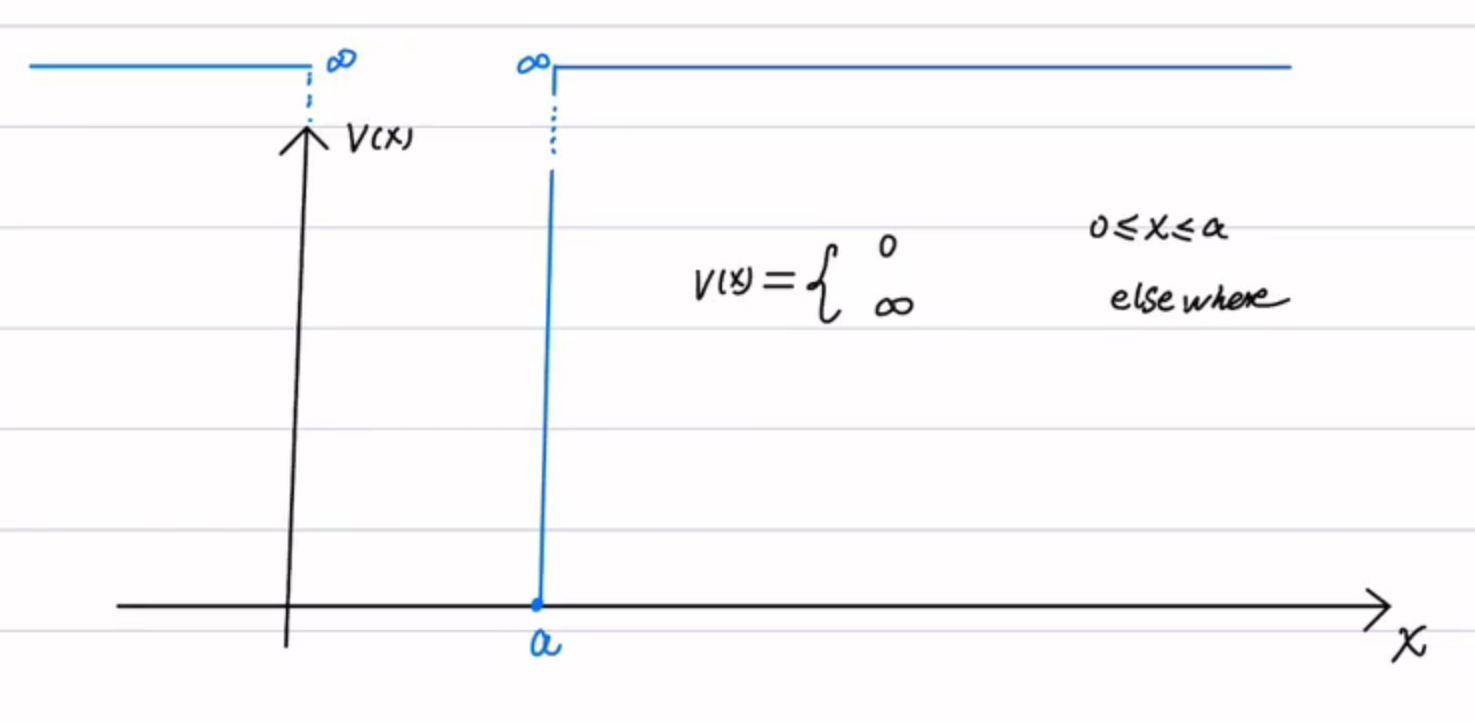
\includegraphics[width=0.7\linewidth]{figure/screenshot0020}
\end{figure}

定态 Schrödinger 方程 (s.e.q.):
\[
\left[-\frac{\hbar^2}{2m}\frac{d^2}{dx^2} + V(x)\right]\varphi(x) = E\varphi(x)
\]

粒子不能存在于势能为 $\infty$ 的区域,因此 $\varphi(x) = 0$ 当 $-\infty < x < 0$ 和 $x > \alpha$。

在 $(0, a)$ 区间 $V(x) = 0$。

\[
-\frac{\hbar^2}{2m}\frac{d^2}{dx^2}\varphi(x) = E\varphi(x)
\]

\[
\frac{d^2}{dx^2}\varphi(x) = \frac{-2mE}{\hbar^2}\varphi(x) \equiv -K^2\varphi(x) \quad \text{其中} \quad K = \sqrt{\frac{2mE}{\hbar^2}}
\]

通解:
\[
\varphi(x) = A e^{i K x} + B e^{-i K x}
\]

或者写成:
\[
A(\cos(Kx) + i \sin(Kx)) + B(\cos(Kx) - i \sin(Kx))
\]

注意到 $A$ 和 $B$ 不过是任意常数。

因此 $A+B$ 和 $iA-iB$ 不过也是另外两个任意常数。

令 $A+B = C$ 和 $iA-iB = D$。

则 $\varphi(x) = C \cos(kx) + D \sin(kx)$。

波函数的一般条件:

\begin{itemize}
	\item $\psi(x)$ 处处单值且连续。
	\item $\frac{d\psi}{dx}$ 在非奇异点处连续。(因为 $\frac{d\psi}{dx}$ 在非奇异点处需要是有限的)
	\item $\psi(x)$ 是有界的。
\end{itemize}

由波函数连续性:

\begin{equation*}
	\psi(0_-) = \psi(0_+) \quad \text{①}
\end{equation*}

\begin{equation*}
	\psi(a_-) = \psi(a_+) \quad \text{②}
\end{equation*}

由1得:
\[
C\cos(k \cdot 0) + D\sin(k \cdot 0) = 0
\]
\[
\Rightarrow C = 0
\]

由2得:
\[
D\sin(ka) = 0
\]

\(D\) 不能也为 0,否则就是平庸解。只能是 \(\sin(ka) = 0\)。

\[
\Rightarrow k = \frac{n\pi}{a}
\]

则
\[
E_n = \frac{\hbar^2 k^2}{2m} = \frac{n^2 \pi^2 \hbar^2}{2ma^2}
\]

这里我们定义一个系统中能量最低的态为基态,往上依次为第一激发态。

\[
\psi_n(x) = D\sin\left(\frac{n\pi x}{a}\right)
\]

为满足归一化条件:
\[
\int_0^a \left|D\sin\left(\frac{n\pi x}{a}\right)\right|^2 dx = 1
\]
\[
\Rightarrow D = \sqrt{\frac{2}{a}}
\]
则
\[
\psi_n(x,t) = \sqrt{\frac{2}{a}} \sin\left(\frac{n\pi x}{a}\right) e^{-iE_n t/\hbar}
\]

我们可以看出,一维无限深方势阱问题中:

\begin{enumerate}
	\item 能量本征函数是分立的,正交归一性由 $\langle \psi_m | \psi_n \rangle = \delta_{mn}$ 来描述。
	\item 能量本征函数是完备的,$(0, a)$ 上的任意函数都可用其展开:
	\[
	\langle x | \psi(t=0) \rangle = \sum_n | \psi_n \rangle \langle \psi_n | \psi(t=0) \rangle = \sum_n C_n \psi_n(x)
	\]
	\item 由本征态构成的 Hilbert 空间维数为 $\infty$,因为 $n$ 可以取到 $\infty$。
	\item 本征函数关于势阱中心奇偶交替。
	\item 基态无节点,第一激发态有 1 个节点,第二激发态有 2 个节点,以此类推。
	\item 一维无限深方势阱无简并。
	\[
	E_n = \frac{n^2 \pi^2 \hbar^2}{2ma^2}
	\]
	其中 $\Delta E_n$ 表示能级差。
	
	\item 随着 $n$ 的增大,相邻能级差 $\Delta E = E_{n+1} - E_n$ 越来越小,当 $ma$ 非常大时趋向于连续分布(对应原理)。
	
	\item 能级相对间隔
	\[
	\frac{\Delta E_n}{E_n} = \frac{\left[(n+1)^2 - n^2\right] \frac{\pi^2 \hbar^2}{2ma^2}}{n^2 \pi^2 \frac{\hbar^2}{2ma^2}} = \frac{2}{n}
	\]
	因此当 $n \rightarrow \infty$ 时,能级相对间隔 $\rightarrow 0$,能量趋向于连续变化。
\end{enumerate}

\subsection{三维无限深方势阱}
对于区域 $0 < x < a$, $0 < y < b$, $0 < z < c$,势能函数定义为:
\[
V(x,y,z) = 
\begin{cases} 
	0 & \text{elsewhere.} \\
	\infty & \text{elsewhere.}
\end{cases}
\]

三维动量算符 $\hat{P} = -i\hbar\nabla$。

在势阱内有定态 Schrödinger 方程 (S.E.):
\[
-\frac{\hbar^2}{2m} \nabla^2 \Psi(x,y,z) = E \Psi(x,y,z)
\]
展开为:
\[
-\frac{\hbar^2}{2m} \left( \frac{\partial^2}{\partial x^2} + \frac{\partial^2}{\partial y^2} + \frac{\partial^2}{\partial z^2} \right) \Psi(x,y,z) = E \Psi(x,y,z)
\]

令 $\Psi(x,y,z) = \psi(x) \phi(y) \varphi(z)$,则有:
\[
-\frac{\hbar^2}{2m} \left( \frac{\psi''(x)}{\psi(x)} + \frac{\phi''(y)}{\phi(y)} + \frac{\varphi''(z)}{\varphi(z)} \right) = E
\]

这可以分解为三个独立的方程:
\[
-\frac{\hbar^2}{2m} \frac{\psi''(x)}{\psi(x)} = E_x, \quad -\frac{\hbar^2}{2m} \frac{\phi''(y)}{\phi(y)} = E_y, \quad -\frac{\hbar^2}{2m} \frac{\varphi''(z)}{\varphi(z)} = E_z
\]
其中 $E_x + E_y + E_z = E$。


\begin{align*}
	-\frac{\hbar^2}{2m} \frac{\varphi''_x(x)}{\varphi_x(x)} &= E, \\
	-\frac{\hbar^2}{2m} \frac{\varphi''_y(y)}{\varphi_y(y)} &= E, \\
	-\frac{\hbar^2}{2m} \frac{\varphi''_z(z)}{\varphi_z(z)} &= E,
\end{align*}

其中 $E_x + E_y + E_z = E$.

可以看出三个方向分别满足一维无限深方势阱的定态 Schrödinger 方程 (S.E.)。

则
\begin{align*}
	\varphi_x(x) &= \sqrt{\frac{2}{a}} \sin\left(\frac{n_x \pi x}{a}\right), & E_x &= \frac{n_x^2 \pi^2 \hbar^2}{2ma^2}, \\
	\varphi_y(y) &= \sqrt{\frac{2}{b}} \sin\left(\frac{n_y \pi y}{b}\right), & E_y &= \frac{n_y^2 \pi^2 \hbar^2}{2mb^2}, \\
	\varphi_z(z) &= \sqrt{\frac{2}{c}} \sin\left(\frac{n_z \pi z}{c}\right), & E_z &= \frac{n_z^2 \pi^2 \hbar^2}{2mc^2},
\end{align*}

\[
\Psi(x, y, z) = \varphi_x(x) \varphi_y(y) \varphi_z(z)
\]
\end{document}